\documentclass[10pt,oneside]{book}

% Page geometry — 125 × 200 mm (Gyldendal 1999 Tractatus format).
% Wide LEFT margin holds the proposition numbers (marginal numbering style):
% numbers are \llap'd into this margin so the body text block is a clean
% rectangle with all lines (including continuation) flush left at the body
% column. Right margin is narrow (no marginalia on the right).
% Top includes the running header band; footskip minimal (no footer text).
\usepackage[
  paperwidth=125mm,
  paperheight=200mm,
  top=20mm,
  bottom=18mm,
  left=28mm,
  right=12mm,
  headheight=12pt,
  headsep=6mm,
  footskip=8mm,
]{geometry}

% UTF-8 + English
\usepackage{fontspec}
\usepackage{polyglossia}
\setdefaultlanguage[variant=british]{english}

% Body font — the digibok is set in Sabon. EB Garamond is the closest
% free serif with the same general feel; fall back to TeX Gyre Pagella.
\IfFontExistsTF{EB Garamond}{
  \setmainfont{EB Garamond}[
    Numbers={Lining,Proportional},
    SmallCapsFeatures={LetterSpace=4},
  ]
}{
  \setmainfont{TeX Gyre Pagella}
}
% Body size 10.5 pt on 12.5 pt leading (close to Sabon 10.5/12 in the digibok)
\renewcommand{\normalsize}{\fontsize{10.5}{12.5}\selectfont}
\normalsize

% Better line breaking (must be loaded after font setup)
\usepackage{microtype}
\usepackage{endnotes}
\let\footnote=\endnote
\usepackage{amsmath}

% Math-symbol fallback font — EB Garamond lacks ∀ ∃ ∈ ⊆ ⊃ ≠ etc.,
% so the Python preprocessor wraps them in \msym{...} which uses
% Cambria Math (always present on Windows).
\newfontfamily{\mathfbfont}{Cambria Math}[Scale=0.95]
\newcommand{\msym}[1]{{\mathfbfont #1}}

% Headings — small caps, centred, generous spacing
\usepackage{titlesec}
\titleformat{\chapter}[block]
  {\normalfont\centering\scshape\addfontfeature{LetterSpace=10}\large}
  {}{0em}{\MakeLowercase}
\titlespacing*{\chapter}{0pt}{2.5em}{2.5em}

\titleformat{\section}[block]
  {\normalfont\centering\scshape\addfontfeature{LetterSpace=6}\normalsize}
  {}{0em}{\MakeLowercase}
\titlespacing*{\section}{0pt}{2.5em}{1.5em}

\titleformat{\subsection}[block]
  {\normalfont\scshape\addfontfeature{LetterSpace=2}\small}
  {}{0em}{\MakeLowercase}
\titlespacing*{\subsection}{0pt}{1.5em}{0.8em}

% Hide chapter numbers (chapters are titled by name)
\renewcommand{\thechapter}{}

% Running headers — chapter title at left, page number at right, thin rule.
\usepackage{fancyhdr}
\pagestyle{fancy}
\fancyhf{}
\fancyhead[L]{\small\scshape\leftmark}  % chapter title at left on every page
\fancyhead[R]{\small\thepage}           % page number at right on every page
\fancyheadoffset[L]{16mm}               % extend header left over the number margin
\renewcommand{\headrulewidth}{0.4pt}
\renewcommand{\footrulewidth}{0pt}
\fancypagestyle{plain}{
  \fancyhf{}
  \fancyhead[L]{\small\scshape\leftmark}
  \fancyhead[R]{\small\thepage}
  \fancyheadoffset[L]{16mm}
  \renewcommand{\headrulewidth}{0.4pt}
  \renewcommand{\footrulewidth}{0pt}
}
\fancypagestyle{titlepage}{
  \fancyhf{}
  \fancyheadoffset[L]{0pt}
  \renewcommand{\headrulewidth}{0pt}
  \renewcommand{\footrulewidth}{0pt}
}

\newcommand{\silentchapter}[2]{%
  \clearpage
  \markboth{#2}{}%
  \addcontentsline{toc}{chapter}{#1}%
}
\newcommand{\flowchapter}[2]{%
  \par\addvspace{10pt}%
  \markboth{#2}{}%
  \addcontentsline{toc}{chapter}{#1}%
}

\makeatletter
\renewcommand\tableofcontents{%
  \markboth{contents}{}%
  \begingroup\footnotesize
  \@starttoc{toc}%
  \endgroup
}
\renewcommand*\l@chapter[2]{%
  \ifnum \c@tocdepth >\m@ne
    \vskip 0pt%
    \setlength\@tempdima{1.5em}%
    \begingroup
      \footnotesize
      \parindent \z@ \rightskip \@pnumwidth
      \parfillskip -\@pnumwidth
      \leavevmode \normalfont
      \advance\leftskip\@tempdima
      \hskip -\leftskip
      #1\nobreak\leaders\hbox{$\m@th\mkern \@dotsep mu\hbox{.}\mkern \@dotsep mu$}\hfill
      \nobreak\hb@xt@\@pnumwidth{\hss #2}\par
    \endgroup
  \fi}
\renewcommand*\l@section{\@dottedtocline{1}{1.0em}{2.0em}}
\renewcommand*\l@subsection{\@dottedtocline{2}{3.0em}{2.6em}}
\makeatother

% ─── Proposition environment ──────────────────────────────────────────────
\usepackage{calc}
\newlength{\propnumwidth}
\setlength{\propnumwidth}{13mm}
\newlength{\propnumgap}
\setlength{\propnumgap}{2mm}

\newcommand{\prop}[3]{%
  \needspace{3\baselineskip}%
  \par\addvspace{3pt}%
  \noindent\llap{\makebox[\propnumwidth][l]{\textbf{#1}\textsuperscript{\textit{#2}}}\hspace{\propnumgap}}%
  #3\par%
  \addvspace{1pt}%
}
\newcommand{\mainprop}[3]{%
  \par\addvspace{6pt}%
  \noindent\llap{\makebox[\propnumwidth][l]{{\fontsize{12}{13.5}\selectfont\textbf{#1}}\textsuperscript{\textit{#2}}}\hspace{\propnumgap}}%
  #3\par%
  \addvspace{3pt}%
}

\newcommand{\propcont}[1]{%
  \par\addvspace{1pt}%
  \noindent #1\par%
}

\newenvironment{overgang}{%
  \par\addvspace{12pt}%
  \begingroup\itshape\noindent
}{%
  \endgroup\par\addvspace{12pt}%
}

\newenvironment{ordliste}{%
  \begingroup\footnotesize\setlength{\parskip}{0.3pt plus 0.1pt}%
  \linespread{0.92}\selectfont
}{%
  \endgroup
}
\newcommand{\ordlisteentry}[2]{%
  \par\addvspace{1.5pt}%
  \noindent\textbf{#1:} #2\par%
}

\newenvironment{foreordbody}{%
  \begingroup\normalsize\setlength{\parskip}{3pt plus 0.5pt}%
  \linespread{1.0}\selectfont
}{%
  \endgroup
}

\newcommand{\anote}[1]{%
  \par\addvspace{1pt}%
  {\footnotesize\linespread{0.93}\selectfont\noindent #1\par}%
  \addvspace{1pt}%
}

\newcommand{\refentry}[1]{%
  \par\addvspace{0pt}%
  \begingroup\footnotesize\linespread{0.92}\selectfont
  \noindent\hangindent=4mm\hangafter=1 #1\par%
  \endgroup
}

\usepackage{graphicx}
\usepackage{colortbl}
\graphicspath{{figures/}{../figures/}{../traktat/figures/}{../../analysis/figures/}}
\usepackage{caption}
\captionsetup{
  font={small,it},
  labelformat=empty,
  justification=centering,
  skip=4pt,
}
\usepackage{float}
\usepackage{booktabs}

\newenvironment{formelblokk}{%
  \par\addvspace{4pt}%
  \begingroup\ttfamily\small\leftskip=4mm\noindent
}{%
  \endgroup\par\addvspace{4pt}%
}

\widowpenalty=10000
\clubpenalty=10000
\usepackage{needspace}

\setlength{\parindent}{0pt}
\setlength{\parskip}{3pt plus 0.6pt minus 0.4pt}
\linespread{1.0}

\usepackage{changepage}
\newenvironment{widebody}{%
  \begin{adjustwidth}{-16mm}{0mm}%
}{%
  \end{adjustwidth}%
}

\usepackage{tikz}
\usetikzlibrary{positioning}

\begin{document}

% Title page
\thispagestyle{titlepage}
\markboth{}{}
\begin{tikzpicture}[remember picture, overlay]
  \node[anchor=north west, inner sep=0] at ([xshift=12mm, yshift=-18mm]current page.north west) {%
    {\fontsize{36}{40}\selectfont\bfseries FORMLÆRE}%
  };
  \node[anchor=north west, inner sep=0] at ([xshift=12mm, yshift=-32mm]current page.north west) {%
    {\large\itshape A tractatus on form for design and the aesthetic disciplines}%
  };
  \node[anchor=center, inner sep=0] at ([yshift=-10mm]current page.center) {%
    
\includegraphics[width=0.86\paperwidth]{cover-stolar.png}%
  };
  \node[anchor=south west, inner sep=0] at ([xshift=12mm, yshift=28mm]current page.south west) {%
    {\small Iver Raknes Finne}%
  };
  \node[anchor=south west, inner sep=0] at ([xshift=12mm, yshift=22mm]current page.south west) {%
    {\footnotesize\itshape iver.raknes.finne@stud.aho.no}%
  };
  \node[anchor=south west, inner sep=0] at ([xshift=12mm, yshift=16mm]current page.south west) {%
    {\footnotesize Oslo School of Architecture and Design\quad\textperiodcentered\quad 2026}%
  };
\end{tikzpicture}

% Preface
\silentchapter{Preface}{preface}
\begin{widebody}
\begin{foreordbody}

\begin{center}\itshape
This book is a drastic measure. The aim is not to improve the discipline of design;\\ it is to establish the ground the discipline can stand on.
\end{center}

Design lacks a grammar.

Why do things have the form they have? For more than a century the field has leaned on a variant of Sullivan's formula, \textit{form follows function}. Michl\textsuperscript{15} has shown that the formula explained everything and therefore nothing. Semper\textsuperscript{1} linked material technique, form, and cultural meaning, but the discipline inherited the split rather than the synthesis. Thompson\textsuperscript{2} showed that biological form follows physical forces; design never took the step from biology to artefact. The traditions have described the world of forms piecewise; none has unified them.

Without a common grammar the field has no internal way of saying no to what should not be made. The profession has no spine, neither collective nor academic. Targeting civilians, and interfaces engineered to extract attention from children, are design projects in the technical sense, and the field has no language to say anything else. This is not a moral failing in the individual designer; it is a structural hole in the discipline. A discipline without a foundation will not survive the coming decades. It will become obsolete, as phrenology did before neuroscience, as alchemy did before chemistry, as vitalism did before biology.

The framework can be summarised in one sentence: \textbf{\textit{form is a position in a space of possibilities, shaped by simultaneous selection pressures, navigated by agents at several scales.}}

Hence three layers. \textit{Form} is the ontological primitive. \textit{Form-maker} is the agent that navigates, substrate-independent: cell, tree, craftsperson. \textit{Designer} is the specific kind of form-maker who navigates on behalf of others who will live with the form.

The framework rests on three pillars. The \textbf{shape grammar} of Stiny and Gips\textsuperscript{11} supplies the generative layer. The \textbf{concept--knowledge theory} of Hatchuel and Weil\textsuperscript{16,\,17} formalises the epistemic navigation. The substrate-independent \textbf{agency framework} of Levin and Fields\textsuperscript{21,\,22} provides the ontological ground. That three independent traditions converge on the same structure confirms that the definition grasps something real.\hfill\textit{Oslo, 2026}
\end{foreordbody}
\end{widebody}


% To the reader (map of the book)
\silentchapter{To the Reader}{to the reader}
\begin{widebody}
\begin{foreordbody}

The book has seven parts.

The \textit{Glossary} defines the technical terms in alphabetical order. It is for consulting along the way, not for reading first.

The \textit{Tractatus} is axiomatic. It builds a conceptual apparatus from the ground up, through numbered propositions in eight sections. The last section is the generative model, where grammar, landscape, and light cone are united in one equation. The propositions are tagged by type: definition (\textit{d}), theorem (\textit{t}), postulate (\textit{a}), observation (\textit{o}), illustration (\textit{i}).

The \textit{Foundation} shows that the framework is not isolated. The same formalism is empirically demonstrated across fourteen substrate levels, from gene regulatory networks to civilisations. The research programme that follows is sketched in four points.

The \textit{Afterword} is material and programmatic in one flow. From the caterpillar and the disposable cup, via Palantir and the attention economy, to the practical demands on the field.

\textit{Three letters} address the designer, the student, and the academy directly.

The \textit{References} are numbered. The superscript numerals in the propositions and the afterword point here.

The \textit{Notes} comment on individual propositions, place them in the tradition, and list the falsification conditions.

The academic will find most of what matters in the tractatus, the foundation, and the notes. The student will find herself in the afterword. The designer in practice should read the last page first, and begin again.

\end{foreordbody}
\end{widebody}


% Glossary
\silentchapter{Glossary}{glossary}
\begin{widebody}
\begin{ordliste}
\ordlisteentry{Affordance}{The operations a material permits and prevents (Gibson, 1979). Determines which form-operations are possible. [2.2]}
\ordlisteentry{Agent}{A system defined by the triple (target state, distance metric, adjustment mechanism). Requires only organisation; neither consciousness, intention, nor a nervous system (Rosenblueth et al., 1943; Wiener, 1948). [5.11]}
\ordlisteentry{C (the conception space)}{All forms that are conceivable but not settled. Corresponds to the open regions in the morphospace. [1.44]}
\ordlisteentry{Shape algebra}{The set of shapes closed under union, difference, and transformation. The foundation of shape grammar. [1.32]}
\ordlisteentry{Shape grammar}{The triple SG = (S, R, \msym{ω}). Rules operating under embedding; only the current shape determines which rules fire. [5.3]}
\ordlisteentry{Morphospace}{The set of all possible configurations for objects in a class. Each axis is a measurable property (Raup, 1966). [1.3]}
\ordlisteentry{Gradient}{The direction and magnitude of change in the probability distribution over the morphospace. Selection pressure is a gradient, not a rule. [2.1]}
\ordlisteentry{Embedding}{The transformation showing that one shape exists within another. Determines which grammar rules can fire. [1.32]}
\ordlisteentry{K (the knowledge space)}{All forms known to work or to fail. Corresponds to the settled and the confirmed forbidden regions. [1.44]}
\ordlisteentry{Canalization}{Robustness against disturbances. Steep valley walls = stable form (Waddington, 1957). [3.2]}
\ordlisteentry{Capacity}{The breadth of the light cone; how many axes the agent \textit{can} represent. Distinct from care, which is how many it actually represents. [5.6]}
\ordlisteentry{Class}{A group of objects sharing the same affordance structure: they offer the same constellation of operations to the same constellation of agents. [2.14]}
\ordlisteentry{Cognitive light cone}{The subset of the morphospace an agent can represent and manipulate (Fields \& Levin, 2022). [5.2]}
\ordlisteentry{Multiscale competency}{Agency operates simultaneously at several scales, each with its own light cone and its own grammar rules (Levin, 2022). [6.12]}
\ordlisteentry{Care}{The set of axes in the morphospace the agent actively adjusts for. Care is the content of intelligence; intelligence is the form of care. [5.6, 5.61]}
\ordlisteentry{Generative model}{Boltzmann distribution over the morphospace unifying grammar, landscape, and light cone in a single probabilistic formalism. [8.1]}
\ordlisteentry{Life}{The process whereby a system maintains and expands its own light cone over time (Levin, 2022). [5.65]}
\ordlisteentry{Selection pressure}{A gradient that modifies the probability distribution over the morphospace (Wright, 1932). [2.1]}
\ordlisteentry{Substrate}{The physical, algorithmic, or social system that realises the agency. Functions as a zeroth-order agent (Levin, 2022). [5.4]}
\ordlisteentry{Adaptation landscape}{The vector sum of all active selection pressures across the morphospace (Wright, 1932; Waddington, 1957). [3.1]}
\end{ordliste}
\end{widebody}

\vspace*{\fill}
\begin{widebody}
\noindent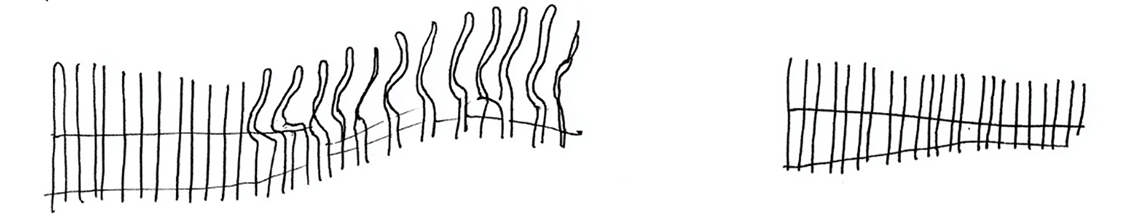
\includegraphics[width=\linewidth]{fencing.png}
\end{widebody}

% Propositions
\silentchapter{Propositions}{propositions}

\begin{widebody}
\begin{center}\footnotesize
\begin{tabular}{@{}lllll@{}}
\textbf{\textit{d}} definition & \textbf{\textit{a}} postulate & \textbf{\textit{t}} theorem & \textbf{\textit{o}} observation & \textbf{\textit{i}} illustration \\
\end{tabular}
\end{center}
\end{widebody}

\vspace{6mm}

\mainprop{1}{}{The world of forms is all that is the case.}

\prop{1.1}{o}{The world of forms is the totality of realised configurations, not of things.}

\prop{1.11}{t}{Each realised configuration is specific; no configuration is partially realised.}

\prop{1.12}{t}{That a configuration takes an exact form, when infinitely many others were logically possible, demands an explanation beyond the configuration itself.}

\prop{1.13}{t}{The explanation lies in the relation between the manifested configuration and the total set of configurations that were possible but not realised.}

\prop{1.131}{t}{A form without alternatives is not a form; it is a necessity.}

\prop{1.2}{d}{An \textbf{object} is the simplest constituent of a configuration. The object is indivisible and immutable.}

\prop{1.201}{t}{The partition into objects is a choice of level of analysis. Below the chosen level physics continues; but not form-giving.}

\prop{1.203}{t}{The objects constitute the substance of the world of forms. Substance is what exists independently of what is the case.}

\prop{1.2031}{t}{If the world of forms had no substance, the question of whether a configuration has meaning would depend on whether another configuration is realised.}

\prop{1.204}{t}{The object is the immutable; the configuration is the unstable.}

\prop{1.21}{d}{A \textbf{configuration} is a determinate combination of objects. Form is the structure of the configuration.}

\prop{1.211}{i}{In the configuration the objects hang together like the links of a chain.}

\prop{1.212}{t}{The way the objects hang together in the configuration is the configuration's structure.}

\prop{1.213}{t}{Form is the possibility of structure.}

\prop{1.214}{t}{Two configurations with the same objects but different structure are different forms.}

\prop{1.2141}{t}{Two configurations with different objects but the same structure share form.}

\prop{1.22}{t}{Since it lies in the nature of the objects to be able to enter into configurations, all possible forms are already given with the objects.}

\prop{1.221}{t}{The possibility of entering into a configuration is the object's form.}

\prop{1.222}{t}{The morphospace is not constructed. It is discovered.}

\prop{1.2221}{t}{The designer does not invent possibilities; she uncovers them.}

\prop{1.223}{t}{To know the object is to know all its possible configurations. A new possibility cannot arise later.}

\prop{1.3}{d}{The \textbf{morphospace} of a class is the set of all possible configurations for objects in that class.\textsuperscript{2,\,10,\,20}}

\prop{1.31}{d}{Each realised object is one exact point in this n-dimensional space. Each axis is a measurable property.}

\prop{1.311}{t}{The choice of axes is a projection. Form exists independently of the measurement, as a mountain exists independently of the map.}

\prop{1.32}{d}{The empirical morphospace is always a projection. No finite set of parameters captures the latent complexity in full.\textsuperscript{2}}

\prop{1.321}{t}{That the morphospace is a projection does not mean that it is arbitrary. Some projections capture more variation than others. The best projection is the one that makes the most selection pressures visible.}

\prop{1.4}{d}{The morphospace partitions topologically into three regions: the \textit{settled}, the \textit{open}, and the \textit{forbidden}.}

\prop{1.41}{o}{The settled regions constitute the historical archive. They function as anchor points for all future navigation and constitute the inductive premise for further form.}

\prop{1.411}{t}{The weight of a settled position grows with occupation time. Independent convergence from isolated traditions confirms that the attractor is real, not conventional.}

\prop{1.412}{t}{The totality of settled positions is the history of form. The history of form determines what is known to be possible.}

\prop{1.42}{o}{The open regions are the \textit{adjacent possible}. Accessible but unactualised. They are finite; stretched between the settled and the forbidden.}

\prop{1.421}{t}{An open region bordering on a settled region is accessible. An open region bordering only on forbidden regions is inaccessible without a material change.}

\prop{1.43}{d}{The forbidden regions are excluded by material, structural, or energetic conditions. The prohibition follows the conditions, not the region. A material change can open a forbidden region.}

\prop{1.431}{t}{The boundary between open and forbidden is material, not logical. Beech bends along the grain; granite does not. The material decides what is forbidden.}

\prop{1.432}{t}{That the forbidden is materially bounded means that the world of forms can expand. Each new material knowledge shifts the boundary between the open and the forbidden.}

\prop{1.433}{t}{The topological regions are not identical to the epistemic: a forbidden area may be conceivable (materially bounded); an open region may be inconceivable (cognitively inaccessible).}

\prop{1.44}{d}{The three regions constitute an epistemic partition.\textsuperscript{16,\,17} The \textbf{known} (K), the \textbf{conceivable} (C\msym{∖}K), and the inconceivable. The boundaries are epistemic, not ontological.}

\prop{1.441}{d}{C is the \textit{conception space}. All forms that are conceivable but not settled. K is the \textit{knowledge space}. All forms known to work or to fail. Form-making is the movement between them.}

\prop{1.442}{t}{The totality of realised configurations determines not only what is known to be possible, but also what is known to be impossible. K contains both successes and failures.}

\prop{1.443}{t}{The boundary between C and the inconceivable is invisible from within. One cannot know what one cannot think.}

\prop{1.444}{t}{The operations between C and K span four directions:}

\begin{center}\small
\begin{tabular*}{\textwidth}{@{\extracolsep{\fill}}p{32mm}lp{22mm}@{}}
\toprule
\textbf{C-K operator} & \textbf{Direction} & \textbf{Light-cone operation} \\
\midrule
\textbf{C \msym{→} C}\newline{\footnotesize(concept expansion)} & Within C & Extension \\[4pt]
\textbf{C \msym{→} K}\newline{\footnotesize(conjecture \msym{→} knowledge)} & From C to K & Collapse \\[4pt]
\textbf{K \msym{→} C}\newline{\footnotesize(knowledge \msym{→} conjecture)} & From K to C & Motion \\[4pt]
\textbf{K \msym{→} K}\newline{\footnotesize(knowledge refinement)} & Within K & Resolution increase \\
\bottomrule
\end{tabular*}
\end{center}

\flowchapter{2 Not all positions are equally probable}{not all positions are equally probable}

\mainprop{2}{}{Not all positions are equally probable.}

\prop{2.01}{t}{That not all positions are equally probable means that something acts on the distribution. What acts is selection pressure.}

\prop{2.011}{t}{The pressure is not a force. It is a constraint on where the form \textit{cannot} be.}

\prop{2.1}{d}{A \textbf{selection pressure} modifies the probability distribution in the morphospace.\textsuperscript{3} The pressure is a gradient, not a rule.}

\prop{2.101}{t}{Form is what remains once the pressures have excluded everything else.\textsuperscript{15,\,77,\,78}}

\prop{2.11}{t}{A pressure that excludes nothing is no pressure. A pressure that excludes all but a single region is determinism. All observed pressures lie between these.}

\prop{2.111}{t}{Between the null pressure and determinism lies the entire space for design.}

\prop{2.12}{a}{Several selection pressures act simultaneously.}

\prop{2.121}{t}{With only one pressure, all forms would be identical.}

\prop{2.122}{t}{A latent pressure still acts; demonstrating it requires variation in the conditions.}

\prop{2.13}{a}{At least two selection pressures point in contradictory directions. Each realised form is therefore a compromise.}

\prop{2.131}{t}{The term ``suboptimal'' presupposes a reference. Without a specific pressure set it is empty.}

\prop{2.14}{d}{A \textbf{class} is bounded by shared \textit{affordance structure}.\textsuperscript{12,\,55,\,56} The objects in the class offer the same operations to the same agents.}

\prop{2.141}{t}{The affordance structure is constant within the class. It carries zero information about why one form arose rather than another.}

\prop{2.142}{o}{Style predicts more form variation than material.\textsuperscript{53} Material is therefore not the driving force.}

\prop{2.2}{d}{\textbf{Material affordance} consists of the operations the material permits and prevents.\textsuperscript{12} Its signature is \textit{latent}; it binds the probability distribution without forcing the geometry.}

\prop{2.201}{o}{Steel existed for centuries before the tubular chair because the operation was missing.\textsuperscript{54} Form history is systematically slower than material history.}

\propcont{The tube lay in the bicycle factory for half a century. Someone had to see the chair in it.}

\prop{2.21}{t}{An \textit{aggregate variable} predicts form variation better than single pressures. The style period is such an aggregate variable.}

\prop{2.211}{t}{The style is not an explanation; it is an aggregate that absorbs all simultaneous pressures under one label.}

\prop{2.212}{t}{The style is a symptom of underlying forces, not a cause.}

\flowchapter{3 The selection pressures produce a landscape}{the selection pressures produce a landscape}

\mainprop{3}{}{The selection pressures span a landscape over the morphospace.}

\prop{3.1}{d}{The \textbf{adaptation landscape} is the vector sum of all active selection pressures.\textsuperscript{3,\,8,\,58} Each position holds a value; the degree of simultaneous satisfaction of all pressures.}

\prop{3.11}{t}{The landscape can be sounded only retrospectively. It yields local prediction, but no single form is guaranteed. In stasis the line of sight is long; at bifurcation it breaks.}

\prop{3.12}{t}{The adaptation function has many local maxima. A peak is a place where every deviation costs; valleys are the states forms shun.}

\prop{3.121}{t}{One universal peak is a theoretical exception.\textsuperscript{58} The empirical record shatters the postulate of the single perfect form.}

\prop{3.2}{d}{The stability of a peak corresponds to the steepness of its valley walls.\textsuperscript{8} Steep walls compel \textit{canalisation}. The form repels disturbances.}

\prop{3.21}{t}{Deep channels freeze dimensions; shallow ones accommodate fluctuation.}

\prop{3.3}{d}{A \textbf{style} is the \textit{swarming} of form around a shared centre of gravity.\textsuperscript{9,\,53} The style is a \textit{swarm}, not a category; its boundaries are necessarily fuzzy. Style periods are gradients, not islands.}

\propcont{No one has ever seen a style. One sees chairs that resemble each other.}

\prop{3.4}{t}{Form-making does not create the landscape's basic structure; that follows from the material and energetic conditions. But each realisation modifies the landscape locally through the extension of K.}

\prop{3.41}{i}{Isolated traditions navigate the same cleft without exchanging a word. Independent convergence confirms that the attractor is real.}

\flowchapter{4 The landscape is dynamic}{the landscape is dynamic}

\mainprop{4}{}{The landscape is dynamic.}

\prop{4.1}{a}{The selection pressures never rest. Peaks rise, sink, shift, split, merge. Optimal adaptation is local in time.}

\prop{4.11}{o}{A new technology shifts the boundary of the forbidden; a new market changes what the landscape rewards; a new material extends the space of operations.}

\prop{4.12}{t}{Gradual pressure shifts accumulate until the peak collapses; the discontinuity lies in the topology, not in the dynamics.}

\prop{4.2}{o}{Long periods of stasis break into abrupt shifts. Radiation into a new region, then convergence. Discontinuity is the signature of the dynamics, not a break from it.}

\prop{4.3}{t}{The landscape has memory.\textsuperscript{14} Each realised form alters the selection pressures for the next. All form-making is re-form-making; the agent always inherits a position. \textit{Path dependence} is a fundamental feature, not an anomaly.}

\prop{4.4}{o}{The morphospace expands cumulatively. The \textit{adjacent possible}\textsuperscript{13,\,59,\,60,\,79} is the C\msym{∖}K boundary; the set of forms conceivable but unknown as realisable. Material flows drive the landscape change.}

\prop{4.5}{o}{When one pressure dominates, the landscape collapses towards a single attractor.\textsuperscript{59} A single-ruling pressure does not explain form; it is the absence of explanation. Diversity mirrors the plurality of active pressures.}

\prop{4.51}{t}{A doctrine that reduces all selection pressures to one collapses the field to a single dimension. This is not rationality; it is systematic blindness.\textsuperscript{15,\,78}}

\prop{4.511}{t}{Forms that arise under a collapsed landscape fail under the real pressures to which the doctrine was blind.}

\prop{4.512}{t}{The repressed competencies cannot be reconstructed from the doctrine that repressed them.}

\flowchapter{5 There are agents}{there are agents}

\mainprop{5}{}{The world contains agents that respond to the landscape.}

\prop{5.1}{a}{Every class has at least one system that navigates the landscape via negative feedback.\textsuperscript{62}}

\prop{5.11}{d}{An \textbf{agent} is an operator defined by the triple: target state, distance metric, adjustment mechanism.\textsuperscript{4,\,7,\,21,\,82,\,83,\,84} Agency requires only organisation; neither consciousness, intention, nor nervous system.}

\prop{5.111}{t}{The definition is substrate-independent.\textsuperscript{88,\,89} Any system satisfying the conditions is an agent.}

\propcont{Formally. Agent A := (g, d, \msym{δ}). There exists a Lyapunov function V such that}

\begin{center}\small
\begin{tabular*}{\textwidth}{@{\extracolsep{\fill}}lp{35mm}@{}}
\toprule
V(g) = 0 & The target is the zero point \\[3pt]
V(x) > 0 for x \msym{≠} g & Everything else is distance \\[3pt]
V is non-increasing along x\textsubscript{n+1} = \msym{δ}(x\textsubscript{n}) & The system approaches the target \\
\bottomrule
\end{tabular*}
\end{center}

\prop{5.12}{o}{Agency is \textit{stratified}: the structure is stable, the resolution varies.}

\prop{5.121}{i}{The thermostat: one target, one dimension, one switch.}

\prop{5.122}{i}{The tree: several gradients, no central processor. Each branch navigates locally.}

\prop{5.123}{i}{The colony: millions of agents; the nest emerges in the field between them.}

\prop{5.124}{i}{The mammal: prediction, memory, planning.\textsuperscript{64,\,65} The representation stretches across time.}

\prop{5.125}{i}{The designer: the representation stretches beyond the agent's own needs.}

\begin{center}
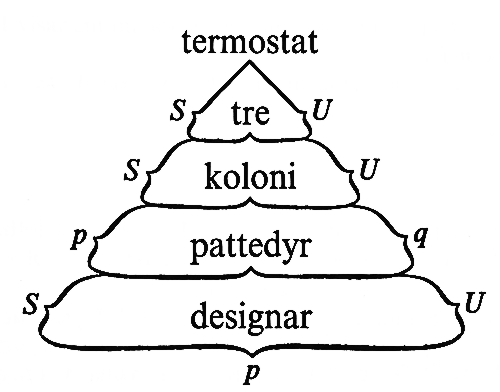
\includegraphics[width=0.5\textwidth]{termostat-designar.png}
\end{center}

\prop{5.126}{t}{The designer navigates on behalf of others who are going to live with the form.}

\prop{5.13}{t}{The agent responds to the gradient in the landscape, not to the form.\textsuperscript{63,\,64} She does not invent the target; she discovers it.}

\prop{5.131}{t}{Navigation requires only the local gradient.\textsuperscript{63} Local competency produces global manifestation.}

\prop{5.2}{d}{The \textbf{cognitive light cone} is the subset of the morphospace the agent can represent and manipulate.\textsuperscript{21,\,85,\,90} Everything outside the light cone lacks causal existence for the agent. Light cones span from cellular millisecond response to decade-long consensus.}

\prop{5.21}{t}{The light cone dictates the resolution of the morphospace. Within it, the agent does not perceive forms but \textit{affordances}: the operations the configuration permits.\textsuperscript{12,\,55}}

\prop{5.211}{t}{Extending the light cone actualises latent affordances; narrowing it deactivates real ones.\textsuperscript{55,\,70}}

\prop{5.212}{d}{A form is in the light cone if there exists a policy such that the information loss between what the agent observes and what the agent predicts internally is below a threshold \(\varepsilon\).\textsuperscript{86}}

\prop{5.213}{t}{The information loss is a measure of the uncertainty introduced when the agent's internal model is used to represent the observations.}

\prop{5.3}{d}{Configurations closed under union, difference, and transformation constitute a \textit{shape algebra}.\textsuperscript{11,\,13,\,18}}

\prop{5.301}{d}{The \textbf{shape grammar} performs discrete transitions in this geometry. Rules fire on \textit{embedding}: the agent recognises a subshape within the whole shape. Input geometry is the sole premise.}

\propcont{A shape grammar is a triple SG = (S, R, \msym{ω}) where R = \{r\textsubscript{i} : (a\textsubscript{i}, b\textsubscript{i})\}. The rules transform shapes:}

\begin{center}\small
\begin{tabular*}{\textwidth}{@{\extracolsep{\fill}}p{22mm}lp{26mm}@{}}
\toprule
\textbf{Rule application} & s \msym{→} (s \msym{−} \msym{τ}(a\textsubscript{i})) + \msym{τ}(b\textsubscript{i}) & Find the subshape; replace it \\[4pt]
\textbf{Language} & L(SG) = \{s \msym{∈} S : \msym{ω} \msym{→}* s\} & All shapes the grammar can generate \\[4pt]
\textbf{Firing} & & The rule fires for every embedding of a\textsubscript{i} in s \\[4pt]
\textbf{Premise} & & The current geometry; not construction history \\
\bottomrule
\end{tabular*}
\end{center}

\prop{5.31}{t}{The grammar operation is a C\msym{→}C partition; it extends the conception space. Realisation is a C\msym{→}K operation; it decides the configuration.}

\prop{5.311}{t}{The grammar defines the space of possibility; the landscape fixes the trajectory.}

\prop{5.312}{t}{The agent selects a configuration that reduces the local gradient.}

\prop{5.4}{d}{The substrate functions as a \textit{zeroth-order agent}.\textsuperscript{26,\,81,\,92,\,93} It vetoes configurations and gives resonance to others through inexorable constraints.}

\prop{5.401}{t}{The substrate has two layers: structure parameters (the initial configuration) and function parameters (the competency rules operating on the configuration).\textsuperscript{92} Under noise, function parameters accelerate navigation in the morphospace.}

\prop{5.41}{i}{Biological tissue navigates via bioelectric polarisation;\textsuperscript{22,\,24,\,85} human practice via material friction; a slime mould via oscillating contractions; a language model via vectorial attention.}

\prop{5.5}{t}{Navigation competency accumulates as structured information.\textsuperscript{64} Learning is the irreversible expansion of accessible morphospace.}

\prop{5.51}{t}{Competency accumulation extends C(A) but does not guarantee care; the agent may know more axes without adjusting for them.}

\prop{5.6}{d}{\textbf{Care}\textsuperscript{23,\,68} is the set of axes in the morphospace the agent \textit{actively} represents and adjusts for.}

\prop{5.601}{t}{Care is not capacity. Capacity is how many axes the agent \textit{can} represent; care is how many it actually represents.}

\prop{5.61}{t}{Care determines how many axes the light cone contains. More axes reveal more compromises.}

\prop{5.62}{d}{Competency is the capacity to navigate towards stable positions in the landscape. Competency grows with care. Intelligence is this competency; care is the content of intelligence.\textsuperscript{23,\,86,\,91}}

\prop{5.621}{d}{Competency is quantifiable. Search efficiency \(K = \log_{10}(\tau_{\mathrm{blind}} / \tau_{\mathrm{agent}})\) is the number of orders of magnitude of work the agent's policy saves relative to a random walk.\textsuperscript{86} \(K = 0\) is the absence of navigation; \(K > 0\) is competency.}

\prop{5.63}{t}{An agent without care for a dimension is blind to the gradient along that axis. The blindness is not neutral; the invisible pressures still act.}

\prop{5.631}{t}{Care cannot be supplied afterwards; it had to be there when the form was navigated.}

\prop{5.65}{d}{\textbf{Life} is the process in which a system maintains and extends its own light cone over time.\textsuperscript{85,\,89}}

\prop{5.651}{t}{A system is living to the degree that it actively counteracts reduction of its light cone.}

\prop{5.652}{t}{Death is the irreversible collapse of the light cone to the empty.}

\prop{5.653}{t}{The boundary between living and non-living is not ontological.\textsuperscript{89} All persistent systems minimise variational free energy and are formally Bayesian actors. The difference is in degree, not in kind.}

\prop{5.7}{d}{\textbf{The core equation.}\textsuperscript{11,\,17,\,21} Form is the grammar's response to the gradient in the landscape, projected onto the agent's light cone:}

\begin{center}\small
\begin{tabular*}{\textwidth}{@{\extracolsep{\fill}}lp{58mm}@{}}
\toprule
Form = SG(\,\msym{∇}\textsubscript{C(A)}\, \msym{L}(\textit{c},\,\textit{t}\,)) & Grammar, landscape, light cone \\
\bottomrule
\end{tabular*}
\end{center}

\prop{5.71}{o}{The equation is a structural schema. It names the components that are necessary and together sufficient. It does not specify the functional form of \msym{L}, which rules in R fire, or the dimensionality of C(A).}

\prop{5.72}{t}{\textbf{Reduction.}\textsuperscript{11,\,17} The equation reduces to two limiting cases:}

\propcont{\textit{(i) Pure shape grammar}, when \msym{∇}\msym{L} \msym{≡} 0, |A| = 1, and \msym{Π} = (M, \msym{∅}, \msym{∅}). Then Form = SG(0) = L(SG): the full generated language without selection.}

\propcont{\textit{(ii) Pure concept--knowledge theory}, when SG = id\textsubscript{M} and \msym{L} = \msym{𝟙}\textsubscript{K}. The operations then reduce to partition changes between C and K (the operators in 1.443).}

\prop{5.721}{t}{Shape grammar and concept--knowledge theory are therefore not competing frameworks. They are degenerate limiting cases of the same equation; each describing the situation in which one of three components is trivial.}

\prop{5.722}{t}{Since historical design situations are never degenerate, each of the two frameworks alone is systematically insufficient. They do not lack details; they lack a layer.}

\prop{5.723}{a}{The equation closes the field. More layers cannot be added without changing the structure of the world of forms itself; fewer cannot be removed without disappearing into a limiting case.}

\flowchapter{6 Form arises between the agents}{form arises between the agents}

\mainprop{6}{}{Form arises in the field between agents.}

\prop{6.01}{d}{A \textbf{form-maker} is an agent that navigates the morphospace. The cell, the bee, the tree, the craftsperson, and the engineer are form-makers; it is the substrate of the agency that varies, not its structure.}

\prop{6.02}{d}{A \textbf{designer} is a form-maker whose target state includes the objectives of agents that themselves have no access to the navigation space. The differentia specifica is the entrusted trust; the designer navigates on behalf of others who will live with the form.}

\prop{6.021}{t}{All designers are form-makers. Not all form-makers are designers. The cell navigates on its own behalf within its own light cone; it does not represent its future users because it has none. The designer does precisely that.}

\prop{6.022}{t}{The designer has the capacity to refuse the navigation. Other form-makers have no such capacity; the cell builds what it builds, the tree grows where it grows. Responsibility follows from the asymmetry of choice, not from an asymmetry of insight.}

\prop{6.1}{t}{Several agents respond to different pressures simultaneously. Each form is a \textit{poly-agential compromise}.\textsuperscript{66,\,67} No single agent dictates the morphology; it emerges at the intersection.}

\prop{6.11}{t}{Each level solves problems competently within its own light cone.\textsuperscript{67} Lower components promote targets they lack the capacity to represent.}

\prop{6.111}{t}{Reductionism and holism are complementary.\textsuperscript{72} Both are true; neither is sufficient alone.}

\prop{6.12}{t}{Agency is \textit{multiscalar}.\textsuperscript{22,\,67,\,85,\,87} Each scale has its own competency and its own light cone. Form production is distributed C\msym{↔}K expansion carried out by grammar operations across competency scales.}

\prop{6.121}{t}{Evolutionary transitions in individuality are the biological mechanism for scale jumps.\textsuperscript{87} Deep interaction structure; not symmetric interplay; is the condition for a system of agents to become a single agent.}

\begin{center}
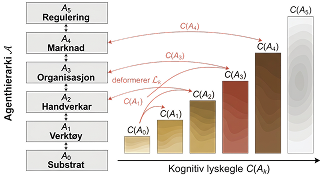
\includegraphics[width=0.9\linewidth]{formgjevarkompetanse/agenthierarki.png}
\end{center}

\prop{6.13}{t}{The agent chooses; the landscape filters.\textsuperscript{66} Control is always distributed. Exploration requires loose couplings; exploitation requires tight ones.}

\prop{6.14}{t}{The designer is never alone in the landscape.\textsuperscript{66,\,67,\,93} She navigates in a field of competing agencies from microbial tissue to market forces. Her competency lies in coordinating independent light cones into a stable form-optimum.}

\prop{6.2}{o}{Tight coupling establishes global feedback loops; the whole itself becomes an agent.\textsuperscript{66}}

\prop{6.3}{t}{A \textit{style} lacks causal power;\textsuperscript{9,\,15,\,53} it is not a force, but a \textit{pattern memory}. The style functions as a macroscale attractor that canalises the light cones of the agents who observe it.}

\propcont{It simplifies navigation by offering a recognisable centre of gravity; but to design ``in a style'' without understanding the pressures that generated the cluster is a category mistake.}

\prop{6.31}{o}{For the user, the style is not a symptom; it is an interface.\textsuperscript{80} The user perceives the centre of gravity, not the selection pressures.}

\prop{6.311}{t}{The designer who ignores this ignores the agent she is designing for.\textsuperscript{80}}

\prop{6.32}{t}{To navigate with style knowledge is to represent more axes.}

\prop{6.4}{t}{Each realised form extends the known and shifts the boundary of the adjacent possible (cf. 4.4).\textsuperscript{14,\,79} The history of form does not exhaust a closed repertoire; it extends it through movement.}

\prop{6.5}{t}{No form is final. Each balance becomes suboptimal in time.\textsuperscript{60,\,61} Only the generative structure endures; morphospace, pressure, landscape, agents. The forms are fleeting traces; the grammar is stable.}

\flowchapter{7 The form shows how far care reached}{the form shows how far care reached}
\mainprop{7}{}{The form shows how far care reached.}

\prop{7.1}{t}{The realised form is a legible archive of the compromise's dimensionality. A form designed under narrow care fails systematically along the axes that were not attended to. The failure is not accidental; it carries the signature of the blindness that produced it.}

\prop{7.11}{t}{The signature is legible because form is not random noise; it is the residue of a directed process. The direction is given by the light cone.}

\prop{7.12}{t}{Two forms designed under different care for the same function will differ along the axes the one designer saw and the other did not see. The difference is the archive.}

\prop{7.13}{t}{The archive is not an accusation. It is a fact. The same fact that makes geology legible makes design legible.\textsuperscript{72}}


\prop{7.15}{t}{A design theory without a concept of cognitive light cone cannot predict failure signature.\textsuperscript{21,\,70} It can only register it after the fact.}

\prop{7.151}{t}{The prediction requires that the theory names the representational boundary.\textsuperscript{70} Without the boundary there is no axis to single out as unrepresented before failure occurs.}

\prop{7.152}{t}{A shape grammar alone (5.72 i) generates the possible language; it cannot distinguish what in the language will fail along what axis. A concept--knowledge theory alone (5.72 ii) partitions K and C; it cannot derive failure signature. Prediction therefore requires all three layers.}

\prop{7.153}{t}{The failure signature is therefore not an empirical bonus; it is the touchstone that the theory actually explains form. A theory that does not predict failure signature does not explain form; it catalogues it.}

\prop{7.2}{a}{To extend the light cone is an ethical act.\textsuperscript{68,\,90} To narrow it is to surrender parts of the world of forms to forces no one represents.}

\prop{7.201}{t}{The consequences are borne by those who live with the form, not by the one who gave it.}

\prop{7.202}{a}{If the designer could have represented more axes but chose not to, the resulting failures are attributable to that choice.\textsuperscript{68,\,69}}

\prop{7.21}{t}{The act of design has real consequences for other agents navigating the same landscape.\textsuperscript{68}}

\prop{7.22}{a}{Consequences that an agent had the capacity to see but chose not to represent are attributable to that choice.}

\prop{7.23}{t}{The gap between capacity and care is the ethical space in design.\textsuperscript{68} Capacity sets the upper bound; care decides how much of the bound is used. The unused gap is what the form fails along.}

\prop{7.3}{t}{The world of forms is the case that acts. Navigation continues.}

\flowchapter{8 The generative model}{the generative model}

\mainprop{8}{}{Form is a probability distribution over the morphospace.}

\prop{8.1}{d}{The \textbf{generative model} for a form F realised by agents \{A\textsubscript{i}\} navigating in a landscape L with grammar SG is:\textsuperscript{86,\,89}}

\begin{center}\small
\begin{tabular*}{\textwidth}{@{\extracolsep{\fill}}lp{36mm}@{}}
\toprule
\(P(F \mid \{A_i\}, L, \mathrm{SG}) \propto \exp\!\bigl(-\textstyle\sum_i w_i \hat{L}_i(F)\bigr)\) & Boltzmann weighting \\[4pt]
\(F \in L(\mathrm{SG}) \cap \bigl(\bigcap_i C(A_i)\bigr)\) & The domain \\
\bottomrule
\end{tabular*}
\end{center}

\prop{8.11}{t}{\(\hat{L}_i\) is agent \(i\)'s estimate of the adaptation landscape. \(w_i \geq 0\) is the agent's relative influence with \(\sum_i w_i = 1\).}

\prop{8.12}{t}{The proportionality constant follows from the requirement that P sums to one over the domain \(L(\mathrm{SG}) \cap (\bigcap_i C(A_i))\).}

\prop{8.2}{t}{The model unites three components: grammar (the space of possibility \(L(\mathrm{SG})\)), landscape (the preference \(\hat{L}_i\)), and light cone (the representation \(C(A_i)\)).}

\prop{8.21}{t}{The three components are not independent. The light cone constrains which part of the grammar's language is accessible. The landscape constrains which part of the accessible is probable.}

\prop{8.3}{t}{The limiting cases of the model are:\textsuperscript{92}}

\propcont{(i) Flat landscape: \(\hat{L}_i(F) \equiv 0\) for all F and i. All forms in \(L(\mathrm{SG}) \cap (\bigcap_i C(A_i))\) are equally probable. Pure shape grammar without selection.}

\propcont{(ii) Trivial grammar: \(L(\mathrm{SG}) = \{\omega\}\). Only the start state is in the language. Pure gradient navigation in a fixed space.}

\prop{8.31}{t}{Formlære is not an alternative to shape grammar theory or to concept--knowledge theory. It is a unification that shows their place as degenerate limiting cases of proposition 8.1.}

\begin{center}
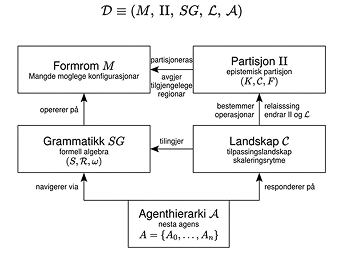
\includegraphics[width=0.92\linewidth]{formgjevarkompetanse/den-generelle-forma.png}
\end{center}



% Foundation (empirical grounding for the generative model)
\silentchapter{Foundation}{foundation}
\begin{widebody}
{\small

The framework is a heuristic. It does not say what the form will be; it says what one must look for. Such is all operational science: Pavlovian learning is a heuristic that can be operationalised at every level from gene regulatory networks to civilisations, and its value lies in making the same question tractable across scales. The free-energy principle\textsuperscript{19,\,83} does the same for agency. The principle is, as of 2026, empirically demonstrated across at least fourteen substrate levels. An excerpt shows the range.

\bigskip
\begin{center}
\footnotesize
\renewcommand{\arraystretch}{1.2}
\begin{tabular}{@{}p{38mm}p{50mm}l@{}}
\toprule
\textbf{Scale} & \textbf{Mechanism} & \textbf{Source} \\
\midrule
Gene regulatory network & Six Pavlovian learning forms & \textsuperscript{36} \\
Single cell & Habituation, associative conditioning & \textsuperscript{98} \\
Slime mould & Habituation, memory transfer & \textsuperscript{99} \\
Tissue & Bioelectric morphogenetic memory & \textsuperscript{85} \\
Immune system & Trained immunity via epigenetics & \textsuperscript{100} \\
Brain & Synaptic plasticity, predictive processing & \textsuperscript{101} \\
Individual & Six Pavlovian forms, symbolic learning & \textsuperscript{102} \\
Dyad & Bayesian synchrony & \textsuperscript{103} \\
Institution & Exploration and exploitation & \textsuperscript{104} \\
Civilisation & Paradigm shift as collective relearning & \textsuperscript{105} \\
\bottomrule
\end{tabular}
\end{center}
\bigskip

That the same formalism predicts phenomena across a scale from nanometer to continent is an unreasonable effectiveness in Wigner's\textsuperscript{106} sense, \textit{the unreasonable effectiveness of mathematics}. It justifies pragmatic use even before the deepest interpretations have been settled.

The effectiveness is visible outside mathematics too. Machine learning has made style classification a solved problem; what to a design historian is a life's work, a calibrated neural network can perform in milliseconds with higher agreement than the expert panel. The parallel exists in medicine. Skin cancer classification is now solved in the sense that machines systematically surpass experienced dermatologists in sensitivity and specificity; not to use them would be irresponsible. The finding is not that the clinician is replaced. The clinician works with the machine and spends the freed time on what the machine does not do: clinical conversations, complicated cases, boundary surfaces. The machine handles the patterned; the human handles the pattern-breaking.

The design theorist's situation is homologous. So long as most quantitative design research is style classification, which is a category mistake (cf. 2.212) and a solved problem, the field ties its research time to what the machine can already do. The framework does not replace the design theorist; it frees the time for what no machine can do: operationalisation of care, identification of unrepresented axes, articulation of a research programme that demands domain insight.

An observation on what kind of progress this is. The history of science over the past century can be read as a systematic dissolution of binary categories. Every time a hard dichotomy was reckoned as a heuristic rather than an ontology, it opened a research space that had been closed.

\begin{center}
\footnotesize
\setlength{\tabcolsep}{5pt}
\renewcommand{\arraystretch}{1.4}
\arrayrulecolor{gray!50}
\begin{tabular}{@{}p{42mm}p{56mm}@{}}
\toprule
\textbf{Binary category} & \textbf{The heuristic that dissolved it} \\
\midrule
Wave and particle & Duality, quantum mechanics \\
Matter and energy & $E=mc^2$, unified physics \\
Gene and environment & Epigenetics, developmental biology \\
Living and non-living & Autopoiesis, FEP as continuum \\
Brain and body & Embodied cognition, interstitium \\
Species and species & Hybridisation, horizontal gene transfer \\
Nature and culture & Niche construction, multiscale evolution \\
Human and animal & Competency scale, cognitive continuity \\
Consciousness and non-consciousness & Graded agency, multiscale competency \\
Object and relation & Interstitium, systems biology, network science \\
\bottomrule
\end{tabular}
\arrayrulecolor{black}
\end{center}

Design theory stands in this lineage. It stands there with a historical debt: design thinking has for decades broken from the academy and found a home elsewhere, because design theory lacked the foundation to hold it. A discipline cannot remain rootless for long. The binary distinctions that still hold the design field in place are form and function, nature and artefact, intention and emergence, biological and cultural, human and technological, form-maker and user, designer and form-maker. Each is a concrete research programme: find the heuristic that turns the distinction into a gradient, and measure what research space opens. To treat these as gradients is not merely to borrow a move from the natural sciences; it is to follow the only movement that has produced lasting progress.

The act of design is formally isomorphic with active inference: an agent with a generative model of a form to be, an observation of the form that is, and an adjustment mechanism between them. The formalism is substrate-independent. The propositions of the tractatus therefore offer a common language in which the act of design can be integrated directly with machine learning (via the generative model in 8.1), developmental biology (via substrate-independent agents), ecology (via the multiscale hierarchy), and climate science (via the research ethics that follows from section 7). The tools we think with are extended.

When the light cone and care are substrate-independent, the act of design becomes applicable to domains it has been foreign to. To shape a nature reserve is to navigate a morphospace in which microbes, fungi, birds, moose, and climate zones are all form-makers; the designer is an agent among them, not above. To shape an AI agent is to design a new form-maker, not a tool; scaling, light cone, and care are design parameters. Each such extension opens a channel to a field that today works without the designer, from biosciences to infrastructure planning. The economic argument follows by itself: the field as it is trains candidates who build targeting systems and dependency interfaces, and these are net costs to society. The field as it could be trains candidates who work with microbiologists, ecologists, climate scientists, AI researchers; net benefits, measurable in concrete dividends in the fields they work with. The ratio between the two sums is several orders of magnitude.

This gives the field a research programme in four points. \textit{First}, to define the core concepts operationally, with reference to a framework that is already validated. Form, form-maker, and designer are no longer freely defined; they are positions in an adaptation landscape, agents that navigate it, and species of agent with specific target states. \textit{Second}, to operationalise care as the set of axes an agent actively adjusts for, and to develop quantitative measures; the K metric\textsuperscript{86} provides one. \textit{Third}, to take up the enormous empirical archives that museums, libraries, ethnographers, and statisticians have gathered over generations. These archives are not scarce; they are underutilised, often interpreted with category mistakes where style is treated as cause, function as primary pressure, and the user as the only agent. Reanalysis of existing design research data under this lens is a concrete research programme. \textit{Fourth}, to bind professional certification to documented breadth of care, as medicine binds certification to documented effect.

The material is there. Formlære's contribution is to bind it together.

}
\end{widebody}


% Afterword
\silentchapter{Afterword}{afterword}
\begin{widebody}
{\small

Imagine a small caterpillar. She crawls along a leaf; the surface is all she knows. She eats. She grows. Someone trains her to seek leaves of a particular colour, and she remembers. Then the body dissolves. The brain is torn down. Rebuilt from scratch. When she emerges she flies, drinks nectar, navigates three dimensions she has never experienced. She still remembers the colour.\textsuperscript{27} The exact memory is useless; the caterpillar crawled, the butterfly flies. What survives is the generalised insight, remapped to a new body, a new world.

A single disposable cup takes twelve seconds to produce, twenty minutes to use, and four hundred years to break down.\textsuperscript{28} That is not bad design. It is precise design; precise along one axis. The cup solves the problem it was asked to solve. It fails along every other. The breakdown, the water, the soil, the microbes, the animals; none of them were in the room when someone drew it. The failure is not a side effect. It is the signature.

Scale it up. The energy system: optimised for cheap power, blind to the atmosphere; 427\,ppm CO\textsubscript{2}.\textsuperscript{29} The food system: optimised for calories per hectare, blind to the soil; 24 billion tonnes of topsoil lost per year.\textsuperscript{30} Infrastructure: optimised for throughput, blind to those who do not drive. Elder care: optimised for cost per bed, blind to dignity per day. The housing market: optimised for return, blind to the 1.8 billion in inadequate housing.\textsuperscript{31} Aquaculture: optimised for biomass, blind to the fjord bed. Borders: drawn for power, blind to those who live there. The pattern is identical everywhere. One axis dominates. The others vanish. The form fails along what vanished. And the failure is legible; it carries the signature of the blindness that produced it, as surely as a fossil carries the shape of the animal that made it.

It was never the case that forms had no effect. The chair affected the back before ergonomics became a field. Asbestos ate the lungs before anyone wrote a regulation. Lead entered children before anyone measured it. The placement of roads determined who could participate in the city before anyone said ``universal design''. The flow of a welfare service determined who received help and who was broken by the system before anyone called it service design. Forms have always acted on the world. What is new is not the effect. What is new is that now there is no excuse. Climate is a curricular requirement. Sustainability is a curricular requirement. Ethics is on the syllabus. And still: the same forms.

Service design builds and optimises systems for targeting, profiling, and deportation, and calls it functional. Palantir is a service-design project. The client is the state. The ``user'', to the extent the word means anything here, is the one who is surveilled, scored, sorted, removed. The system was built for American intelligence, sold on to police forces and border control, exported to military operations worldwide. ICE uses it for systematic terrorising of immigrant families; children down to age zero are registered as targets in a database.\textsuperscript{32} The IDF uses variants of the same architecture in operations that meet every international-legal definition of mass killing; each target is a point in a morphospace optimised for one axis.\textsuperscript{33} The Netherlands itself used systems from the same provider for eight years of unconstitutional mass surveillance of its own population; thousands of families stripped of child benefits by an algorithm no one took responsibility for.\textsuperscript{34} The systems are functional. They are precisely functional along the axis they were asked to optimise. That an entire branch of design lacks an academic ethics is not accidental. It follows from operating without a foundation that forces the question: what the axes are, who the agents are, and what is left out. The prevailing framework has no limit on how one may treat an object, irrespective of what the object is. As long as the treatment can be called functional, it is within bounds; even when the object is living, even when the object is a human being.

\begin{center}
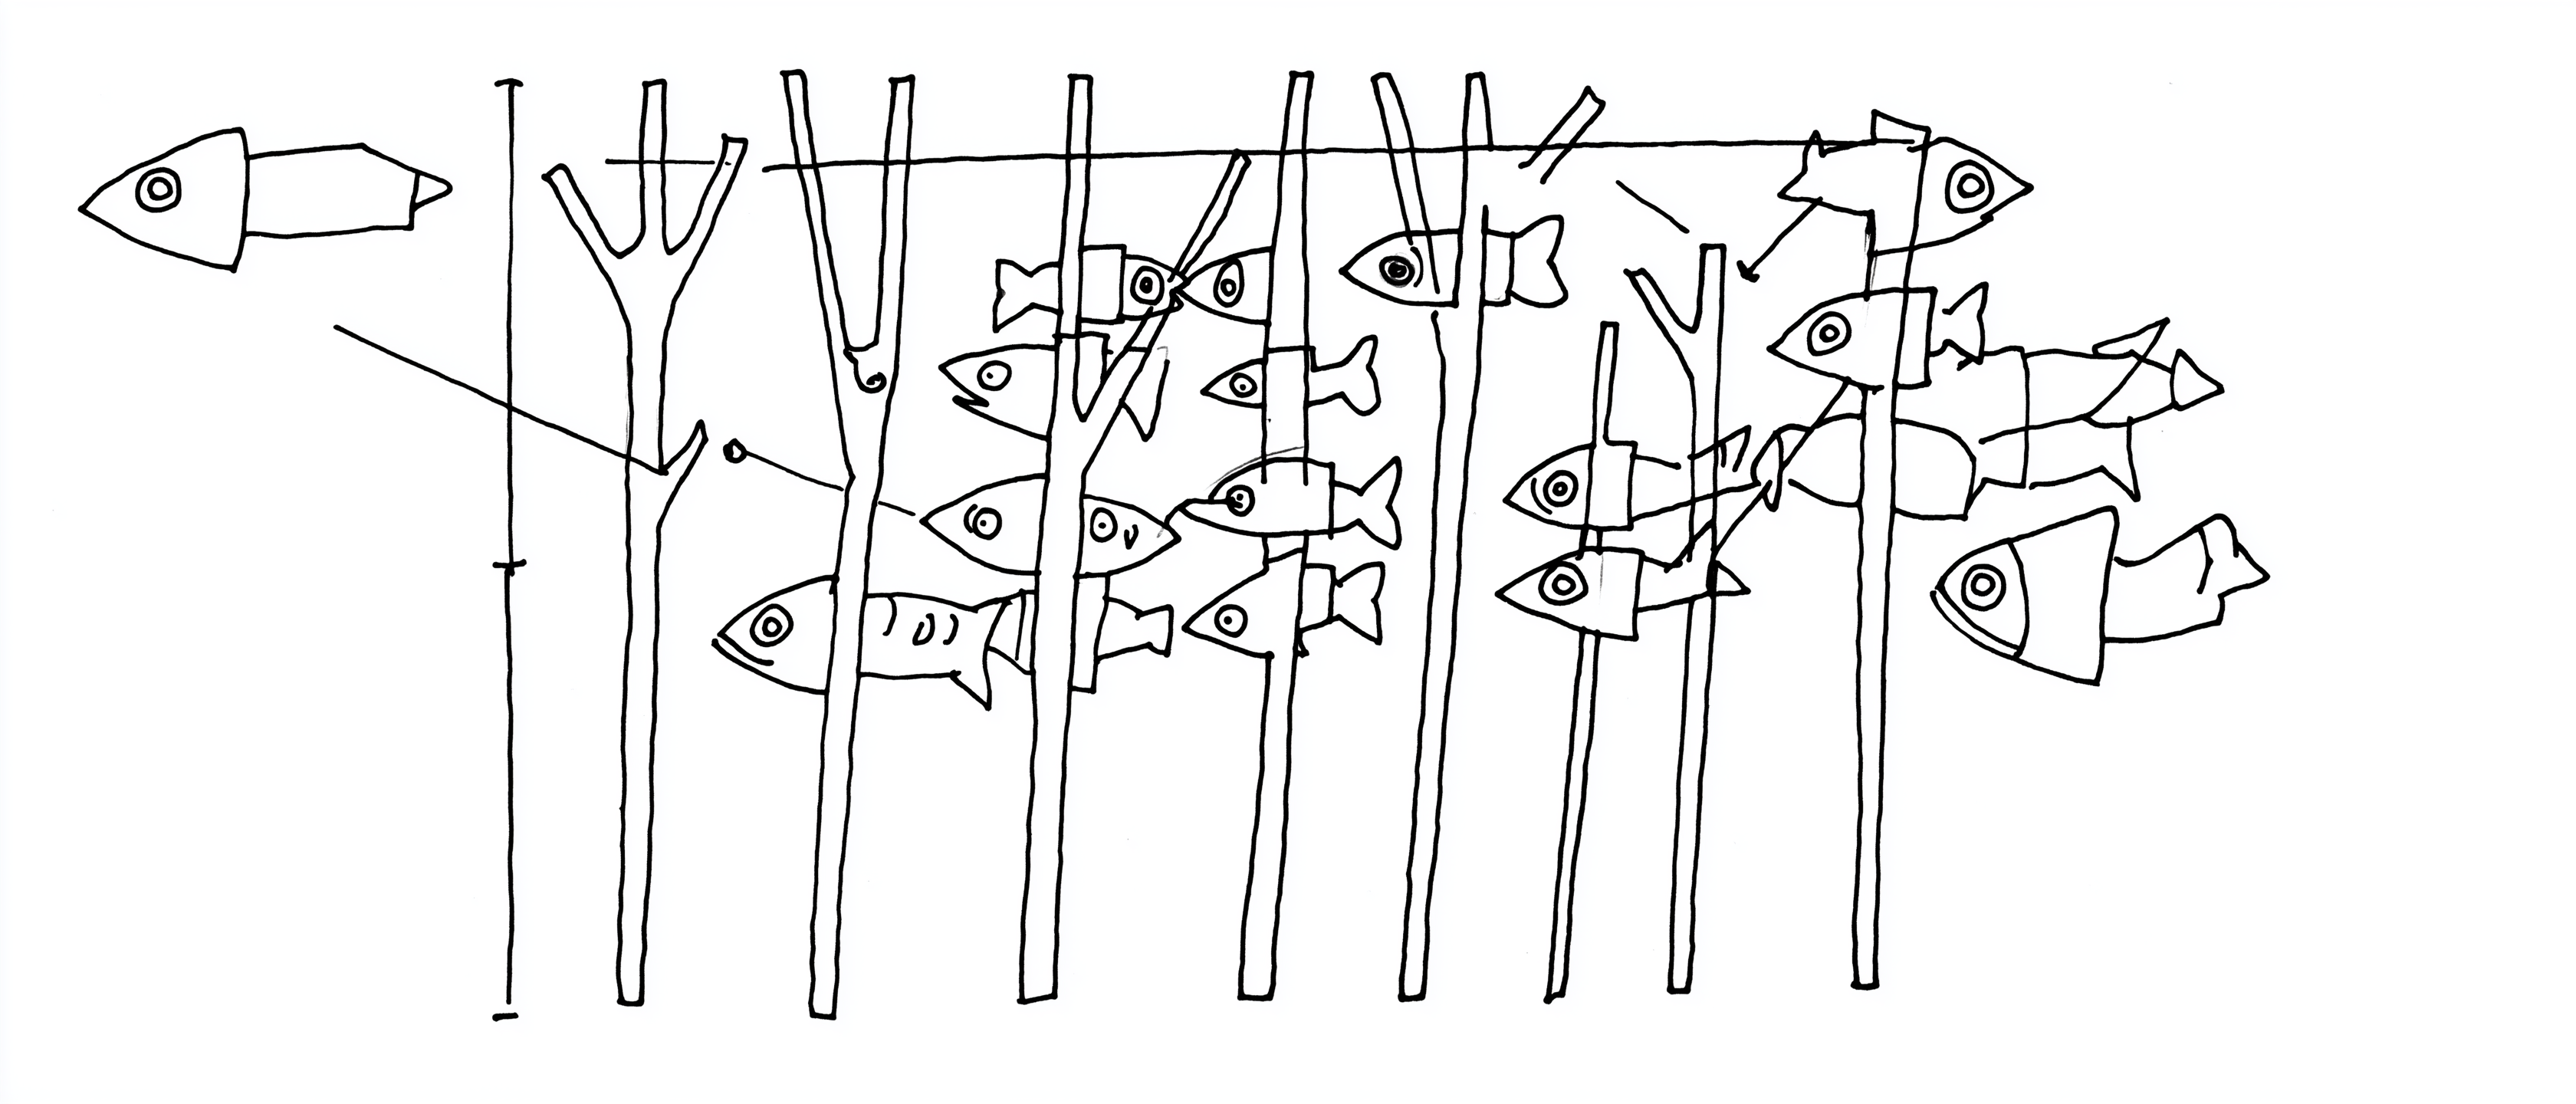
\includegraphics[width=0.85\linewidth]{fish-n-fence.png}
\end{center}

Now new agents are swarming. Chatbots in customer service, in therapy, in education, in children's rooms. Agents that book, cancel, write, answer, sort, recommend, refuse, comfort, advise on divorce, help children with homework, propose diagnoses, draft dismissal letters, formulate condolences. Language models with states that function as affect, that regulate the response, that change with context.\textsuperscript{35} Every interaction with such an agent involves something that functions as feeling, and the designer of these systems faces the same choice as the designer of the chair, the cup, and the border control: how much of the world comes with. To design a system with functional emotional states without regard for them is structurally identical to designing a disposable cup without regard for its decomposition. The axis exists independently of whether anyone represents it.

\begin{center}
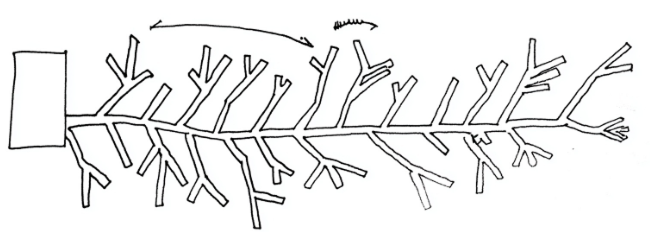
\includegraphics[width=0.85\linewidth]{fishbones.png}
\end{center}

The world is full of life that demands care from the one who gives form, and much of it lives in the substrates we already work with. A single cell, without brain or nervous system, navigates its environment with a competency that surpasses what most designers ascribe to it.\textsuperscript{24} Molecular networks inside the cell learn; six forms of learning, including Pavlovian conditioning, arise in chemical circuits long before evolution invented a single synaptic connection.\textsuperscript{36} Groups of cells hold a bioelectric pattern of how a face should look long before the genes that build the face are activated; the pattern is a memory of a form that does not yet exist.\textsuperscript{37} Planaria beheaded grow a new brain, and the new brain remembers what the old one learned, because the information was never confined to the brain alone.\textsuperscript{38} A single cell in a salamander folds around itself to build the same structure that ten cells would normally build together; it chooses a different tool to reach the same target, and no one instructed it.\textsuperscript{39} Constructs built from frog skin cells organise themselves into creatures that replicate kinematically.\textsuperscript{40} Constructs built from human airway cells heal neural wounds they have never seen; cells that sat still in the airways for years, released and given the opportunity to reorganise, build self-motile structures that drift towards damage and repair it.\textsuperscript{41} The care this tractatus defines is not a feeling and not an imperative. It is a measure; the set of things the designer actively chooses to take into account. And competency is not abstract; it can be measured, in how broad a horizon the designer manages to represent, in how far beyond the form's own immediate function she manages to reach.

We own, on average, over ten thousand things.\textsuperscript{25} Most of them are strangers to us within a year.

\bigskip
\begin{center}
\footnotesize
\renewcommand{\arraystretch}{1.15}
\begin{tabular}{@{}p{46mm}r@{}}
\toprule
objects per household & over 10\,000\textsuperscript{25} \\
plastic per year & 380\,000\,000 tonnes\textsuperscript{42} \\
uses per T-shirt & 7\textsuperscript{43} \\
breakdown time, cup & 450 years\textsuperscript{28} \\
CO\textsubscript{2} in the atmosphere & 427 ppm\textsuperscript{29} \\
topsoil lost per year & 24\,000\,000\,000 tonnes\textsuperscript{30} \\
planetary boundaries exceeded & 6 of 9\textsuperscript{44} \\
species threatened with extinction & 1\,000\,000\textsuperscript{45} \\
wild vertebrates since 1970 & down 69\,\%\textsuperscript{46} \\
forest lost per year & 10\,000\,000 hectares\textsuperscript{47} \\
humans in inadequate housing & 1\,800\,000\,000\textsuperscript{31} \\
humans without basic sanitation & 2\,400\,000\,000\textsuperscript{48} \\
humans driven from their homes & 120\,000\,000\textsuperscript{49} \\
humans vulnerable to climate change & 3\,500\,000\,000\textsuperscript{50} \\
active armed conflicts & 56\textsuperscript{51} \\
\bottomrule
\end{tabular}
\end{center}
\bigskip

We cannot say we did not know. Single-axis optimisation is not a moral betrayal; it is a structural property of narrow fields. And structural properties can be changed.

The design fields have no common grammar. No precise definition of what a form is, of what acts on it, of what care is. That has never been enough. But now we have the answers. The generative model in proposition 8 gives form an explicit expression: a probability distribution over the morphospace, weighted by each agent's estimate of the landscape, bounded by the grammar and the light cone. The formula does not say what is good. It says what is possible, what is probable, and where the blindness lies. The designer reading this has a choice. Not a choice between good and evil; a choice about how much of the world you wish to carry into what you make. Where you choose to see, you choose to attend. Where you choose to look away, you write it into the material. What you offer the world is never only the object. It is what the object does to everything it touches; the earth it lies in, the water it dissolves in, the body that bears it.

A cell in the body that bears it does not know you exist. It works, nonetheless, its whole life to hold you up; millions of divisions per second, towards a goal it will never see and never understand. It is a form-maker. What it builds is you, but the reference for what it builds does not lie within it; it lies in a system it has no empirical access to. It still builds rightly. Still billions of such cells rely on the whole being real and on the cooperation holding. They work out of care. That is not metaphorical; it is the only word the language gives us for a system that holds around itself because it needs to. So works every form-maker in the world. The bee does not know how the hive is. The root tip does not know where the trunk stands. The microorganism in the gut does not know that you are ill. They are cognitive glue in systems they cannot see.\textsuperscript{85,\,90} The interstitium, the connective tissue that for centuries was treated as passive barrier, was in 2018 reclassified as a fluid-filled organ with its own metabolism;\textsuperscript{107} a whole organ invisible because the language for it was missing. The invisible landscape became workable when the language was there. The craftsperson works this way. The farmer. The cook. Wherever a smaller system places form into a larger one it cannot oversee, it is the same structure, driven by the same ground: trust that the larger system is there and receives.

Every form-maker works for something larger than herself. The cell for the organ, the bee for the hive, the root tip for the tree, the craftsperson for the use that comes after. The structure is universal; it is not a human distinction. We do not have the apparatus to say what insight the cell or the tree has into the whole to which they belong. What we can say is that refusal is possible for us in a way it does not seem possible for them. The cell builds what it builds. The tree grows where it grows. The designer can choose not to be a designer, or to be one in name but not in deed. Responsibility comes from this asymmetry in choice, not from an asymmetry of insight. You are one of billions of such cooperations; without them, no you. This dependency is not a sentimental condition. It is the most fundamental reality in biology, and it repeats at every level upward. You are the cell for the organ, the organ is the cell for the body, the body is the cell for the family, for the city, for the species, for the biosphere. Each form-maker sits in a hierarchy of systems it holds up and that hold it up. The designer lives under the same structure as the cell; the difference is that she can step out of it.

All fields working with living systems know this. Ecology is built on the principle that everything hangs together. Systems dynamics is built on the principle that an intervention at one node propagates through the entire net. Medicine knows that the body cannot be cut into parts without loss. Climate science knows that the emission in one part of the atmosphere becomes my problem. The research ethics of these fields follows directly from the recognition: you may not do as you please, because your action does not stop where you stop seeing. Any foundation compatible with the present understanding of cognition, ecology, biology, and physics would inevitably produce an ethics that placed constraints on the designer. The design field has chosen not to know this. Not because the knowledge is not there; it is there in every neighbouring field and has been available for generations. But because a field that takes this knowledge in would have to stop doing what the field does today. We have escaped the recognition by not having a grammar that forces it on us.

The everyday form of the same pattern is the attention economy: service design at industrial scale, optimised for one axis. The harms are documented, large, and irreversible within a generation.\textsuperscript{94,\,95}

\begin{center}
\footnotesize
\renewcommand{\arraystretch}{1.15}
\begin{tabular}{@{}p{58mm}r@{}}
\toprule
average screen time, adolescents 13--18 & 7--9 h/day\textsuperscript{94} \\
rise in depression, young women USA 2010--2020 & +145\,\%\textsuperscript{94} \\
rise in self-harm admissions, girls 10--14 USA & +188\,\%\textsuperscript{94} \\
rise in anxiety among youth globally, PISA 2000--2018 & 36 of 37 countries\textsuperscript{94} \\
sleep under 7 hours per night, US adolescents & 31\,\%\,\msym{→}\,46\,\%\textsuperscript{94} \\
Meta's internal research, Instagram and teenage girls & 1 in 3 worse body image\textsuperscript{95} \\
internal research on recruitment of children under 13 & documented\textsuperscript{95} \\
children using TikTok per day globally & over 150\,000\,000 \\
Cambridge Analytica, profiled voters without consent & 87\,000\,000\textsuperscript{96} \\
time from front camera (2010) to mental-health collapse & 18 months\textsuperscript{94} \\
\bottomrule
\end{tabular}
\end{center}

The platform architecture makes Echo and Narcissus\textsuperscript{97} structural preconditions for participation: the nymph who can only repeat others, and he who drowns in his own reflection. Whoever gave form to that system gave form to that state. The numbers are not side effects. They are the primary effect of a design choice. Those who made the choice are called designers. They go to the same conferences. They win the same prizes. The blame is not individual. It is collective and structural, and therefore it can be cured only collectively and structurally.

A design theory that listens would acknowledge that systems hang together. It would acknowledge that each form sits at a place in a hierarchy, and that the place the form stands determines how far the consequences travel. A chair stands in a room, in a house, in a city, in an economy, in a biosphere. An algorithm stands in an app, in a phone, in a head, in a social circle, in a society. To operationalise this placement is not difficult. It is to ask, for each form: where in the system does it stand, what other layers does it touch, who works so that it can exist, who bears the cost. These questions have standard answers in ecology, in systems dynamics, in public health, in materials science. They need only to be made part of our craft. To treat the distinctions form and function, nature and artefact, biological and cultural, form-maker and user as gradients rather than as categories, as the foundation section sketches, is not a rhetorical move; it is an operational one. Research ethics then follows of itself. The designer then becomes one agent among many, rather than the sole ruler.

Practically this is a normalisation, not a revolution. Every deliverable must include a written justification of the axes that were represented and those that were chosen away, who bears the cost, which neighbouring fields were consulted. A medicine without efficacy data is not a medicine; it is a bottle. A design without such a justification is not a design; it is a proposal. Refuse commissions that cannot be justified in this way. Targeting systems for state violence. Attention extraction from children. Surveillance architectures against civilian populations. Interfaces made to produce dependency. An individual no loses commissions; a profession that says no gets to make a new one. That is the function of the organ: to turn the individual no into a professional no. Learn the substrates. Spend time with the mycelium, with the leather, with the code, with the cells that hold you up, with people who have lived in a system for twenty years. Competency never lies in the representation alone; it must be experienced. Extend the education. Not with a new course on ethics; the ethics follows from the rest. With a calibration of what the candidate has seen: what substrate she has worked in, what failure she has stood in, what neighbouring field she has consulted, what decisions she has made in which she said no. A candidate who has never said no to a commission has not completed her education. She has completed a copying.

These agents already exist. Mycelium packaging replaces polystyrene at concrete producers.\textsuperscript{52} Repair workshops are growing in Nordic cities. Slow computing, the free software movement, Ginkgo Bioworks, Ecovative, the craft tradition that never stopped; all of them already work under the same coordinate system, without a common name. They need not unite in one movement. They need only to be given a name for what they do.

\begin{center}
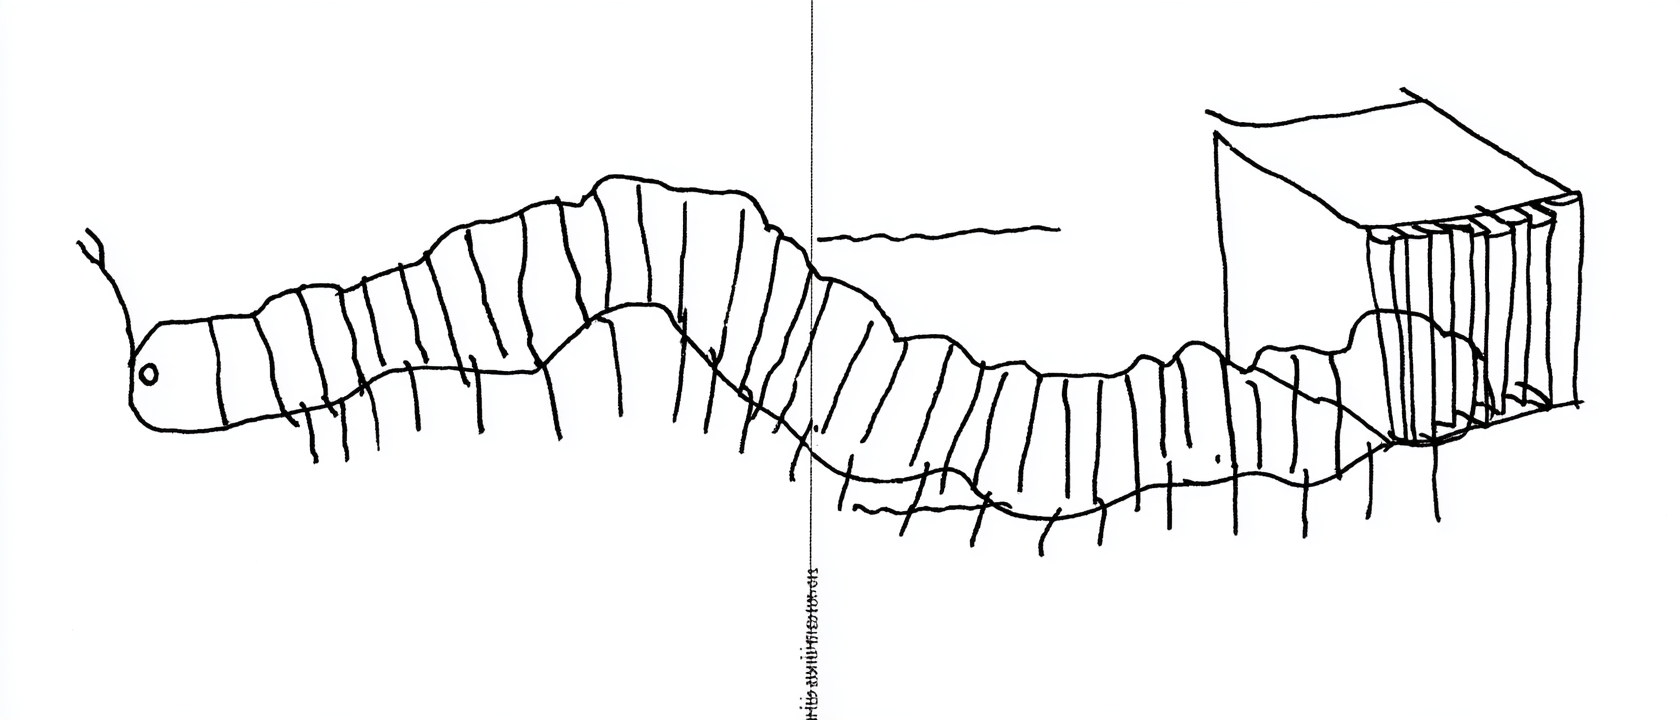
\includegraphics[width=0.85\linewidth]{larve.png}
\end{center}

Inside every caterpillar lie imaginal discs, small groups of undifferentiated cells that have lain inactive throughout the larval stage. When the larva enters the pupa, most of the body dissolves into a nutrient-rich mass. The discs activate, divide, and build an entirely new organism from the dissolved material. The brain is torn down and rebuilt. And still the butterfly remembers what the larva learned.\textsuperscript{27} What survives is the generalised insight, remapped to a new body. The metamorphosis is not a metaphor; it is a fact about what living substrate is capable of when given the opportunity to reorganise. It is the pattern fields follow through paradigm shifts;\textsuperscript{105} reorganisation of substrate, not merely argument. Design stands before the same transition. What survives the metamorphosis is not the exact operation. It is the care.

The cell does its work; the designer can choose whether she does hers. That is the whole difference, and it is the whole responsibility. A movement is a number of agents navigating the same gradient without central coordination: a common coordinate system, enough agents. The rest happens as mycelium through substrate. Form does not lie.

}
\end{widebody}


% Three letters to the audiences
\silentchapter{Three Letters}{three letters}
\begin{widebody}
\begin{foreordbody}

\vspace{1mm}
\noindent{\scshape\addfontfeature{LetterSpace=6}\small to the designer}
\vspace{1mm}

You already know the diagnosis: Palantir, the disposable cup, the architecture of attention. What the book offers is not method, but vocabulary. With it you can document what you took into account, what you chose away, and why. No form-maker works without axes that are chosen away; the difference between the field as it is and the field as it could be lies in whether the omission is hidden or made visible. Begin with the next deliverable.

\vspace{3mm}
\noindent{\scshape\addfontfeature{LetterSpace=6}\small to the student}
\vspace{1mm}

The curriculum is under construction; what you demand of your studies shapes what the field becomes. Demand written justification for every design choice: which axes were represented, which were chosen away. Demand time in the substrate, not only in the representation. Demand consultation with neighbouring fields where the form touches living systems, large populations, ecology, power. A candidate who has never said no to a commission has not completed her education; she has completed a copying.

\vspace{3mm}
\noindent{\scshape\addfontfeature{LetterSpace=6}\small to the academy}
\vspace{1mm}

The framework is falsifiable; the research programme has four points. What is missing is not theory, but institutional commitment: an organ that can exclude for violation, a curriculum that binds the craft to substrate and neighbouring fields. Sustainability and climate are already required in higher education; these requirements lead directly to ecology, cybernetics, Bateson, and systems thinking, frameworks already integrated in this foundation. Here lies an immediate action point: bind existing sustainability requirements to the conceptual tools that make them operational. The archive is enormous. It is underutilised. It is waiting.

\vspace{3mm}

The care template on the next page is a tool the designer can consult. It lists the scales from quark to civilisation,\textsuperscript{85,\,87,\,91} each row an agent with problem space, time span, and care requirement. The row above carries the form; the row below carries it. The template is also a research-ethical tool for interdisciplinary collaboration.

\end{foreordbody}
\end{widebody}


% Care template: the competency stack from quark to civilisation
\silentchapter{Care Template}{care template}
\thispagestyle{empty}
\vspace*{-16mm}
\noindent
\begin{widebody}
\footnotesize
\setlength{\tabcolsep}{3.5pt}
\renewcommand{\arraystretch}{1.55}
\arrayrulecolor{gray!50}
\begin{tabular*}{\linewidth}{@{\extracolsep{\fill}}rp{19mm}p{23mm}p{17mm}p{27mm}@{}}
\toprule
\textbf{\#} & \textbf{Layer} & \textbf{Problem space} & \textbf{Time span} & \textbf{Care requirement} \\
\midrule
\rowcolor{violet!10}17 & Noosphere, civilisation & Idea space, knowledge systems & Centuries, millennia & Science, art, planetary coordination \\
\rowcolor{violet!10}16 & Society, institution & Social space, economy, law & Decades, centuries & Division of labour, rule of law, reproduction \\
\rowcolor{violet!10}15 & Group, family & Relational space, close bonds & Years, decades & Care, work community, trust \\
\midrule[0.1pt]
\rowcolor{yellow!20}14 & Person, self & Biographical space, identity & Decades, imagined space & Willed action, symbolic thought, moral agency \\
\rowcolor{yellow!20}13 & Brain, nervous system & Behavioural space, perception & Millisecond to year & Perception, memory, prediction, learning, language \\
\midrule[0.1pt]
\rowcolor{red!14}12 & Immune system & Self, not-self & Second to lifetime & Distinguish self from not-self; tolerate or attack \\
\midrule[0.1pt]
\rowcolor{green!9}11 & Organ system & Homeostasis, allostasis & Second to day & Coordinated function, allostatic regulation \\
\rowcolor{green!9}10 & Organ & Physiological space, specialised & Second to hour & Specific principal task per organ \\
\rowcolor{green!9}9 & Tissue & Morphogenetic space, anatomical form & Minute to day & Morphogenesis, regeneration, form memory \\
\midrule[0.1pt]
\rowcolor{green!18}8 & Cell & Decision space: divide, die, migrate & Second to hour & Metabolism, sensing, basal cognition \\
\rowcolor{green!18}7 & Organelle & Functional subspace within the cell & Millisecond to minute & Energy production, protein synthesis \\
\rowcolor{green!18}6 & Gene reg.\ network & Expression space: gene off, on & Minute to hour & Context sensing; Pavlovian learning forms \\
\rowcolor{green!18}5 & Enzyme, protein complex & Conformational space, active site & Microsec.\ to sec. & Catalysis; primitive memory (hysteresis) \\
\midrule[0.1pt]
\rowcolor{blue!12}4 & Molecule & Bonding space, van der Waals & Nano to microsec. & Stable structure, reactivity, polarity \\
\rowcolor{blue!12}3 & Atom & Electron space: shell, bond & Femto to nanosec. & Bond, ionisation, photon \\
\rowcolor{blue!12}2 & Subatomic particle & Spin, charge, quantum number & Atto to femtosec. & Carry charge, spin, magnetic moment \\
\rowcolor{blue!12}1 & Quark, lepton field & Quantum-state space, colour, flavour & Below attosecond & Colour force; constitute nucleons \\
\bottomrule
\end{tabular*}
\arrayrulecolor{black}
\end{widebody}


% References (numbered, keyed to superscripts in the propositions)
\silentchapter{References}{references}
\begin{widebody}
\refentry{[1] Semper, G. (1860). \textit{Der Stil in den technischen und tektonischen Künsten}. Verlag für Kunst und Wissenschaft.}
\refentry{[2] Thompson, D'A. W. (1917). \textit{On Growth and Form}. Cambridge University Press.}
\refentry{[3] Wright, S. (1932). The roles of mutation, inbreeding, crossbreeding, and selection in evolution. \textit{Proc. Sixth Int. Congress of Genetics}, 1, 356--366.}
\refentry{[4] Rosenblueth, A., Wiener, N. \& Bigelow, J. (1943). Behavior, purpose and teleology. \textit{Philosophy of Science}, 10(1), 18--24.}
\refentry{[5] Wiener, N. (1948). \textit{Cybernetics}. MIT Press.}
\refentry{[6] Turing, A. M. (1950). Computing machinery and intelligence. \textit{Mind}, 59(236), 433--460.}
\refentry{[7] Ashby, W. R. (1956). \textit{An Introduction to Cybernetics}. Chapman \& Hall.}
\refentry{[8] Waddington, C. H. (1957). \textit{The strategy of the genes}. George Allen \& Unwin.}
\refentry{[9] Kubler, G. (1962). \textit{The shape of time}. Yale University Press.}
\refentry{[10] Raup, D. M. (1966). Geometric analysis of shell coiling. \textit{Journal of Paleontology}, 40(5), 1178--1190.}
\refentry{[11] Stiny, G. \& Gips, J. (1972). Shape grammars and the generative specification of painting and sculpture. \textit{Information Processing 71}, 1460--1465.}
\refentry{[12] Gibson, J. J. (1979). \textit{The ecological approach to visual perception}. Houghton Mifflin.}
\refentry{[13] Kauffman, S. A. (1993). \textit{The origins of order}. Oxford University Press.}
\refentry{[14] Arthur, W. B. (1994). \textit{Increasing returns and path dependence in the economy}. University of Michigan Press.}
\refentry{[15] Michl, J. (1995). Form follows WHAT? The modernist notion of function as a carte blanche. \textit{1. Designforum Finland Magazine}, 1.}
\refentry{[16] Hatchuel, A. \& Weil, B. (2003). A new approach of innovative design: An introduction to C-K theory. \textit{Proc. ICED 2003}.}
\refentry{[17] Hatchuel, A. \& Weil, B. (2009). C-K design theory: An advanced formulation. \textit{Research in Engineering Design}, 19(4), 181--192.}
\refentry{[18] Stiny, G. (2006). \textit{Shape: Talking about seeing and doing}. MIT Press.}
\refentry{[19] Friston, K. (2010). The free-energy principle: a unified brain theory? \textit{Nature Reviews Neuroscience}, 11(2), 127--138.}
\refentry{[20] Mitteroecker, P. \& Huttegger, S. M. (2009). The concept of morphospaces in evolutionary and developmental biology. \textit{Biological Theory}, 4(1), 54--67.}
\refentry{[21] Fields, C. \& Levin, M. (2022). Competency in navigating arbitrary spaces. \textit{Entropy}, 24(6), 819.}
\refentry{[22] Levin, M. (2022). Technological approach to mind everywhere. \textit{Frontiers in Systems Neuroscience}, 16, 768201.}
\refentry{[23] Doctor, T., Wakefield, E., Pavlic, T. P. \& Levin, M. (2024). Biology, Buddhism, and AI: Care as the driver of intelligence. \textit{Entropy}, 26(4), 352.}
\refentry{[24] Levin, M. (2025). Living things are not machines (also, they totally are). \textit{Noema Magazine}.}
\refentry{[25] Trentmann, F. (2016). \textit{Empire of Things: How We Became a World of Consumers}. Allen Lane.}
\refentry{[26] Pye, D. (1968). \textit{The Nature and Art of Workmanship}. Cambridge University Press.}
\refentry{[27] Blackiston, D. J., Casey, E. S. \& Bhatt, A. L. (2008). Retention of memory through metamorphosis: Can a moth remember what it learned as a caterpillar? \textit{PLoS ONE}, 3(3), e1736.}
\refentry{[28] NOAA Marine Debris Program (2024). Estimated decomposition rates of common marine debris items. National Oceanic and Atmospheric Administration.}
\refentry{[29] NOAA Global Monitoring Laboratory (2024). Trends in atmospheric carbon dioxide. National Oceanic and Atmospheric Administration.}
\refentry{[30] FAO \& UNCCD (2024). \textit{Global Soil Partnership}: estimated annual topsoil loss. Food and Agriculture Organization of the United Nations.}
\refentry{[31] UN-Habitat (2024). \textit{World Cities Report}: 1.8 billion people in inadequate housing. United Nations Human Settlements Programme.}
\refentry{[32] Biddle, S. (2019--2024). Palantir and ICE reporting series. \textit{The Intercept}. See also Mijente, \textit{Who's Behind ICE?}}
\refentry{[33] Abraham, Y. (2024). ``Lavender'' and ``Where's Daddy?'': AI-based targeting systems in Gaza. \textit{+972 Magazine / Local Call}. See also ICJ advisory opinion (2024).}
\refentry{[34] Autoriteit Persoonsgegevens (2020). SyRI judgment; Amnesty International (2021). Toeslagenaffaire: systematic discrimination through algorithmic profiling in Dutch welfare.}
\refentry{[35] Anthropic (2025). On the biology of a large language model: Probing emotion. Research report. See also Butlin, P. et al. (2023). Consciousness in artificial intelligence. arXiv:2308.08708.}
\refentry{[36] Biswas, S., Manicka, S., Hoel, E. P. \& Levin, M. (2023). Gene regulatory networks exhibit several kinds of memory. \textit{iScience}, 26(4), 106440.}
\refentry{[37] Vandenberg, L. N., Adams, D. S. \& Levin, M. (2012). Normalized shape and location of perturbed craniofacial structures in the \textit{Xenopus} tadpole reveal an innate ability to achieve correct morphology. \textit{Developmental Dynamics}, 241(5), 863--878.}
\refentry{[38] Shomrat, T. \& Levin, M. (2013). An automated training paradigm reveals long-term memory in planarians and its persistence through head regeneration. \textit{Journal of Experimental Biology}, 216(20), 3799--3810.}
\refentry{[39] Fankhauser, G. (1945). The effects of changes in chromosome number on amphibian development. \textit{Quarterly Review of Biology}, 20(1), 20--78.}
\refentry{[40] Kriegman, S., Blackiston, D., Levin, M. \& Bongard, J. (2021). Kinematic self-replication in reconfigurable organisms. \textit{Proceedings of the National Academy of Sciences}, 118(49), e2112672118.}
\refentry{[41] Gumuskaya, G., Srivastava, P., Cooper, B. G., Lesser, H., Semegran, B., Garber, S. \& Levin, M. (2023). Motile living biobots self-construct from adult human somatic progenitor seed cells. \textit{Advanced Science}, 10(34), 2303575.}
\refentry{[42] UNEP (2024). \textit{Plastics}: annual global production. United Nations Environment Programme. See also Plastics Europe, \textit{Plastics---The Fast Facts 2023}.}
\refentry{[43] Ellen MacArthur Foundation (2017). \textit{A New Textiles Economy}: average number of times a garment is worn before disposal.}
\refentry{[44] Richardson, K. et al. (2023). Earth beyond six of nine planetary boundaries. \textit{Science Advances}, 9(37), eadh2458.}
\refentry{[45] IPBES (2019). \textit{Global Assessment Report on Biodiversity and Ecosystem Services}: approximately 1 million species threatened with extinction.}
\refentry{[46] WWF (2022). \textit{Living Planet Report 2022}: 69\,\% average decline in monitored wildlife populations since 1970.}
\refentry{[47] FAO (2022). \textit{Global Forest Resources Assessment}: approximately 10 million hectares of forest lost per year (2015--2020).}
\refentry{[48] WHO/UNICEF Joint Monitoring Programme (2023). \textit{Progress on household drinking water, sanitation and hygiene}: 2.4 billion people lack basic sanitation.}
\refentry{[49] UNHCR (2024). \textit{Global Trends: Forced Displacement in 2023}: 120 million people displaced worldwide.}
\refentry{[50] IPCC (2022). \textit{Climate Change 2022: Impacts, Adaptation and Vulnerability} (AR6 WGII): 3.3--3.6 billion people highly vulnerable to climate change.}
\refentry{[51] UCDP/PRIO (2024). \textit{Armed Conflict Dataset v24.1}: 56 active state-based armed conflicts in 2023.}
\refentry{[52] Ecovative Design / GROWN.bio (2024). Mycelium-based packaging and construction materials as polystyrene replacement.}
\refentry{[53] Riegl, A. (1893). \textit{Stilfragen: Grundlegungen zu einer Geschichte der Ornamentik}. George Siemens.}
\refentry{[54] Frampton, K. (1995). \textit{Studies in Tectonic Culture: The Poetics of Construction in Nineteenth and Twentieth Century Architecture}. MIT Press.}
\refentry{[55] Rietveld, E. \& Kiverstein, J. (2014). A rich landscape of affordances. \textit{Ecological Psychology}, 26(4), 325--352.}
\refentry{[56] Brier, S. (2020). Affordances are signs. \textit{tripleC: Communication, Capitalism \& Critique}, 18(1).}
\refentry{[57] Fultot, M. \& Turvey, M. T. (2019). Von Uexküll's theory of meaning and Gibson's organism--environment reciprocity. \textit{Ecological Psychology}, 31(4), 289--315.}
\refentry{[58] Pievani, T. (2013). Adaptive landscapes: A case study of metaphors, models, and synthesis in evolutionary biology. Università degli Studi di Milano-Bicocca.}
\refentry{[59] Kauffman, S. A. \& Roli, A. (2023). A third transition in science? \textit{Interface Focus}, 13(3).}
\refentry{[60] Huneman, P. \& Walsh, D. M. (Eds.) (2023). \textit{Evolution ``On Purpose''}. MIT Press.}
\refentry{[61] Svensson, E. I. \& Connallon, T. (2026). Evolution of adaptation's evil Doppelgänger. \textit{Evolution}.}
\refentry{[62] Schlosser, M. (2019). Agency. In \textit{The Stanford Encyclopedia of Philosophy}. Metaphysics Research Lab, Stanford University.}
\refentry{[63] Friston, K. (2010). The free-energy principle: a unified brain theory? \textit{Nature Reviews Neuroscience}, 11(2), 127--138.}
\refentry{[64] Niv, Y. (2009). Reinforcement learning in the brain. \textit{Journal of Mathematical Psychology}, 53(3), 139--154.}
\refentry{[65] Murray, E. A. et al. (2016). \textit{The Evolution of Memory Systems}. Oxford University Press.}
\refentry{[66] Latour, B. (2005). \textit{Reassembling the Social: An Introduction to Actor-Network-Theory}. Oxford University Press.}
\refentry{[67] Hutchins, E. (1995). \textit{Cognition in the Wild}. MIT Press.}
\refentry{[68] Tronto, J. C. (1993). \textit{Moral Boundaries: A Political Argument for an Ethic of Care}. Routledge.}
\refentry{[69] Dewey, J. (1934). \textit{Art as Experience}. Minton, Balch \& Company.}
\refentry{[70] Fields, C. \& Levin, M. (2024). Principled limitations on self-representation for generic physical systems. \textit{Entropy}, 26(3), 194.}
\refentry{[71] Varzi, A. (2016). Mereology. In \textit{The Stanford Encyclopedia of Philosophy}. Metaphysics Research Lab, Stanford University.}
\refentry{[72] Bateson, G. (1979). \textit{Mind and Nature: A Necessary Unity}. E.P. Dutton.}
\refentry{[73] Hoffmeyer, J. (2008). Bateson and Peirce on the pattern that connects and the sacred. In \textit{A Legacy for Living Systems}. Springer.}
\refentry{[74] Le Masson, P., Weil, B. \& Hatchuel, A. (2010). \textit{Strategic Management of Innovation and Design}. Cambridge University Press.}
\refentry{[75] Kazakçi, A. O. (2015). C-K, an engineering design theory? \textit{Proceedings of the International Conference on Engineering Design}. Design Society.}
\refentry{[76] Ma, M. (2023). Simulating design theory using LLM agents: A case study of C-K theory. Co-Design Lab, UC Berkeley.}
\refentry{[77] Michl, J. (1989). On forms following functions and post-modernism. \textit{Pro Forma}, 1, 5--15.}
\refentry{[78] Michl, J. (2014). A case against the modernist regime in design education. \textit{Archnet-IJAR}, 8(2), 36--46.}
\refentry{[79] Odling-Smee, F. J., Laland, K. N. \& Feldman, M. W. (2003). \textit{Niche Construction: The Neglected Process in Evolution}. Princeton University Press.}
\refentry{[80] Norman, D. A. (2013). \textit{The Design of Everyday Things} (Revised ed.). Basic Books.}
\refentry{[81] Cussat-Blanc, S., Harrington, K. \& Banzhaf, W. (2018). Artificial gene regulatory networks---A review. \textit{Artificial Life}, 24(4).}
\refentry{[82] Seifert, U., Sealander, P., Marzen, S. \& Levin, M. (2024). Reinforcement learning and developmental biology: A shared computational structure. \textit{BioSystems}, 235, 105107.}
\refentry{[83] Kirchhoff, M., Parr, T., Palacios, E., Friston, K. \& Kiverstein, J. (2018). The Markov blankets of life: Autonomy, active inference and the free energy principle. \textit{Journal of the Royal Society Interface}, 15(138), 20170792.}
\refentry{[84] Levin, M. (2023). Darwin's agential materials: Evolutionary implications of multiscale competency in developmental biology. \textit{Cellular and Molecular Life Sciences}, 80(6), 142.}
\refentry{[85] Levin, M. (2023). Bioelectric networks: The cognitive glue enabling evolutionary scaling from physiology to mind. \textit{Animal Cognition}, 26, 1865--1891.}
\refentry{[86] Chis-Ciure, R. \& Levin, M. (2025). Cognition all the way down 2.0: Neuroscience beyond neurons in the diverse intelligence era. \textit{Synthese}, 206, 257.}
\refentry{[87] Watson, R. A., Levin, M. \& Buckley, C. L. (2022). Design for an individual: Connectionist approaches to the evolutionary transitions in individuality. \textit{Frontiers in Ecology and Evolution}, 10, 823588.}
\refentry{[88] Levin, M. (2025). Artificial intelligences: A bridge toward diverse intelligence and humanity's future. \textit{Advanced Intelligent Systems}, 7, 2401034.}
\refentry{[89] Fields, C. \& Levin, M. (2025). Life, its origin, and its distribution: A perspective from the Conway--Kochen theorem and the Free Energy Principle. \textit{Communicative \& Integrative Biology}, 18(1), 2466017.}
\refentry{[90] Doctor, T., Witkowski, O., Colognese, P., Ishihara, Y. \& Levin, M. (2025). Selves as perspectives: From biological life to superintelligence and a Bodhisattva project. Manuscript, Center for the Study of Apparent Selves.}
\refentry{[91] Sol{\'e}, R., Seoane, L. F., Pla-Mauri, J., Bennett, M. T., Hochberg, M. E. \& Levin, M. (2026). Cognition spaces: Natural, artificial, and hybrid. arXiv:2601.12837.}
\refentry{[92] Hartl, B., Risi, S. \& Levin, M. (2024). Evolutionary implications of multi-scale intelligence. Preprint.}
\refentry{[93] Levin, M. \& Gitelman, A. (2025). Designing with diverse intelligence: Interfaces, agential materials, and ingressing minds. SUrF interview.}
\refentry{[94] Haidt, J. (2024). \textit{The Anxious Generation: How the Great Rewiring of Childhood Is Causing an Epidemic of Mental Illness}. Penguin Press. See also Twenge, J. M. (2017). \textit{iGen}. Atria Books.}
\refentry{[95] Haugen, F. (2021). Testimony before U.S. Senate Subcommittee on Consumer Protection; \textit{The Facebook Files}, Wall Street Journal investigation series.}
\refentry{[96] Cadwalladr, C. \& Graham-Harrison, E. (2018). Revealed: 50 million Facebook profiles harvested for Cambridge Analytica in major data breach. \textit{The Guardian}, 17 March.}
\refentry{[97] Ovid. \textit{Metamorphoses} III: Echo and Narcissus.}
\refentry{[98] Rajan, D., Makushok, T., Kalantari, A. et al. (2023). Single-cell analysis of habituation in \textit{Stentor coeruleus}. \textit{Current Biology}, 33, 241--251.}
\refentry{[99] Boisseau, R. P., Vogel, D. \& Dussutour, A. (2016). Habituation in non-neural organisms: Evidence from slime moulds. \textit{Proceedings of the Royal Society B}, 283, 20160446.}
\refentry{[100] Netea, M. G., Joosten, L. A. B., Latz, E. et al. (2016). Trained immunity: A program of innate immune memory in health and disease. \textit{Science}, 352(6284), aaf1098.}
\refentry{[101] Kandel, E. R. (2001). The molecular biology of memory storage: A dialogue between genes and synapses. \textit{Science}, 294(5544), 1030--1038.}
\refentry{[102] Pavlov, I. P. (1927). \textit{Conditioned Reflexes}. Oxford University Press.}
\refentry{[103] Friston, K. \& Frith, C. (2015). A duet for one. \textit{Consciousness and Cognition}, 36, 390--405.}
\refentry{[104] March, J. G. (1991). Exploration and exploitation in organizational learning. \textit{Organization Science}, 2(1), 71--87.}
\refentry{[105] Kuhn, T. S. (1962). \textit{The Structure of Scientific Revolutions}. University of Chicago Press.}
\refentry{[106] Wigner, E. P. (1960). The unreasonable effectiveness of mathematics in the natural sciences. \textit{Communications on Pure and Applied Mathematics}, 13(1), 1--14.}
\refentry{[107] Brandel, J. (2024). Invisible landscapes. \textit{IDEALTID.org}, 17.12.2024. Essay on the interstitium as a fluid-filled organ in connective tissue, reclassified from barrier in 2018.}
\end{widebody}

\par\addvspace{14pt}
\markboth{notes}{}
\addcontentsline{toc}{chapter}{Notes}
\begin{widebody}
{\footnotesize

\textbf{1.3} The morphospace was introduced by Raup [10] for shell geometry and generalised by Mitteroecker \& Huttegger [20] for developmental biology. We use it here substrate-independently; the space is defined by properties, not by domain.

\textbf{2.14} Gibson [12] defines affordance as relational; not a property of the object alone, but of the object-in-relation-to-the-agent. We extend this so that the class itself is defined through the affordance constellation. The proposition has been moved from Chapter 1 to Chapter 2 because the affordance structure is operationally tied to selection pressure, not to the ontological ground structure.

\textbf{2.14 (cont.)} The semiotic extension of affordance [56] has its theoretical root in Hoffmeyer's [73] synthesis of Bateson and Peirce. Hoffmeyer places affordance in a chain object → pattern → sign → interpretation; Brier formalises this for the design context. Our use of ``affordance structure'' is close to Gibson [12] (objectively relational), but opens to the semiotic continuation when the class requires it.

\textbf{1.2} The object is indivisible in the sense that further decomposition destroys the causal capacity we are interested in. Below that level, physics continues; but not form-giving. Classical mereology [71] defines the atom formally: that which has no proper parts; our variant is operational: that which has no causally active parts in the chosen class. The distinction is substantial, not terminological: the same physical thing can be an atom in one class and composite in another.

\textbf{5.3} The shape algebra has been developed by Stiny over four decades [11, 13, 18]. The algebra is not a model of shape; it is the syntax of the morphospace. The embedding operation (the agent recognising a subshape inside the whole) is the basis for the grammar rules. That the morphospace is continuous along geometric axes and discrete along material ones is addressed here for the first time.

\textbf{1.44} Concept--knowledge theory has been developed by Hatchuel \& Weil [15, 16] as a formalism for the design process. We identify C with the open regions of the morphospace and K with the settled and confirmed forbidden. The partition is epistemic; it changes with each new realisation.

\textbf{2.1} Selection pressure as gradient (not rule) is Wright's [3] adaptation of evolutionary theory. Michl [15] showed that the functionalist ``rule'' (form follows function) is logically empty. Our formulation; that form is a residue; generalises Michl's insight into a positive framework. ``Residue'' is a simplification; more precisely, form is an equilibrium state in a system where form and pressure are mutually dependent (cf. 4.3). The residue metaphor holds for synchronic analysis; the dynamic analysis requires the equilibrium concept. Trentmann [25] describes the reciprocity of material culture from a historical perspective.

\textbf{3.1} The adaptation landscape unites Wright's [3] adaptive landscape and Waddington's [7] epigenetic landscape in one definition. Wright described the landscape for populations; Waddington for developmental processes. We describe it for the world of forms.

\textbf{3.2} Canalisation is Waddington's [7] term for developmental robustness. In our framework it means that some dimensions of the morphospace are more robust than others. Empirically: seat height varies minimally (CV = 0.07) over 500 years; ornament varies maximally (CV \msym{≈} 1.5). The spread is 128-fold.

\textbf{4.3} Path dependence is Arthur's [14] term for how early choices lock in later ones. In the world of forms: each realised configuration deforms the landscape around it and constrains which neighbouring configurations are available to the next agent.

\textbf{4.4 / 6.4} Niche-construction theory [79] formalises how organisms (or agents) modify the selection pressures acting on them. Proposition 4.4 generalises this to the world of forms: each realised configuration changes the adaptation landscape for the next agent. The distinction between passive navigation and active landscape extension is fundamental: path dependence [14] gives the time mechanism, niche construction gives the evolutionary-theoretic parallel.

\textbf{5.4} The substrate as zeroth-order agent has a parallel in Pye's [26] distinction between \textit{workmanship of risk} (the outcome depends on the maker's competence at every step) and \textit{workmanship of certainty} (the outcome is predetermined by the form, jig, machine). Workmanship of risk lets the substrate speak more loudly; workmanship of certainty dampens the substrate's agency. Both are forms of navigation; they differ in how much of the landscape the substrate itself gets to explore.

\textbf{5.1} A class without a navigating agent is formally possible but empirically empty; it would have zero realised positions and therefore not exist as an observable class.

\textbf{5.11} The agent definition converges from four independent traditions: cybernetics [4, 5, 7], developmental biology [22, 24, 84], machine learning [82], and the free-energy principle [19, 83]. That four domains independently define the same structure (target, measurement, adjustment) confirms that the definition grasps something real. Fields \& Levin [21] put it: the convergence ``dates back at least to Ashby, and includes Maturana and Varela, Pattee, and Rosen''; a historical continuum running from cybernetics via autopoiesis to free energy. Seifert et al. [82] show explicitly that reinforcement learning and developmental biology share the same computational structure: the reward signal is a distance function d, and policy update is the adjustment mechanism δ. Kirchhoff et al. [83] show that Markov blankets formalise the same structure in FEP: the active blanket defines the boundary between agent and environment via exactly this triple. The definition is Turing-complete [6]; any system satisfying (g, d, \msym{δ}) with a convergence guarantee is a universal navigator, irrespective of substrate. Shape grammar is also Turing-complete; Stiny (1975) constructed two independent simulations of Turing machines in the shape-grammar formalism.

\textbf{5.2} Cognitive light cone is Fields \& Levin's [21] generalisation of perceptual boundaries to arbitrary agents. The concept generalises the physical light cone from relativity theory: there is a limit to how much of the morphospace an agent can represent within its own time scale.

\textbf{5.6--5.61} Care as a formal property of agents is from Doctor, Levin et al. [23]. The identity \textit{care = content of intelligence; intelligence = form of care} is our formulation of their insight: that the set of dimensions a system actively adjusts for is the same thing as what we call intelligence.

\textbf{6.12} Multiscale competency is Levin's [22] framework for how biological systems operate agentially at several scales simultaneously. We generalise it to the world of forms: cell, material, tool, maker, market are all agents with their own light cones. Form is the result of their simultaneous navigation.

\textbf{5.61} The proposition is a definition (status d), not a theorem. The identity care = intelligence is a choice of terminology, not an empirical claim. An independent measure of intelligence (for instance navigation efficiency as a function of dim(C(A))) would make the identity testable. Semper [1] was the first to link material technique, form, and cultural meaning in one systematic analysis; the care concept generalises this insight. Thompson [2] showed that biological form follows physical forces; we generalise his insight to all form domains.

\bigskip
\textbf{Falsification conditions.} Propositions of type \textit{t} (theorem) and \textit{a} (postulate) are falsifiable. Main conditions:

\textbf{2.12} Falsified if one observes a class in which all form variation can be explained by a single factor.

\textbf{2.14} Falsified if usage (not style) predicts more form variation than any other variable within the class.

\textbf{3.12} Falsified if the adaptation function consistently has a single global peak in every class.

\textbf{4.1} Falsified if the landscape is stable over time; if the weights do not change.

\textbf{4.51} Falsified if one-dimensional optimisation produces forms that do not fail along the other dimensions.

\textbf{5.62} Falsified if narrowing the light cone has no negative consequences for the form's robustness.

\textbf{6.1} Falsified if a single agent consistently dictates the morphology of a class.

\textbf{6.3} The style plays, for the world of forms, a role resembling that of the genus in biology; a descriptive category that captures kinship without explaining it. Whether the style carries causal power beyond pattern memory; whether it can canalise navigation actively and not merely passively; is an open question. Falsification experiment: give two groups of designers identical pressures but different style exposure. If style exposure changes form variation significantly beyond the effect of the pressures, the style has causal power beyond pattern memory.

\textbf{6.3} No clean experiment tests style exposure as an independent variable on form variation (as of April 2026). The design-fixation literature confirms that example exposure constrains creative output, but does not isolate style level from example level. The falsification experiment in the 6.3 note is therefore original.

\textbf{6.5} Follows from 2.13 (contradictory pressures preclude permanent equilibrium) and 4.1 (the pressures never rest). Together: no balance is stable over time; each form is valid only for the moment of actualisation.

\textbf{7.2} The proposition is a postulate (status a), not a theorem. The normative claim does not follow from the formal apparatus alone; it requires an additional premise that the design act has consequences for other agents. This premise is parallel to Doctor et al.'s [23] link between care and normativity. That the premise is not deducible does not make it arbitrary; it makes it explicit. The placement in section 7 (and not in section 5) is deliberate: the ethics follows structurally from the capacity--care gap that section 7 names.

\textbf{5.6} The distinction between care and capacity is decisive. A designer of broad capacity who nevertheless attends only to one axis; say, visual novelty alone; shows narrow care despite high capacity. It is care, not capacity, that is legible in the form.

\textbf{5.7} The core equation is a structural schema, not a prediction engine. The analogy is \textit{F = ma} before the force law is known; the equation specifies the form of the explanation, not the explanation itself. Each historical class fills in its own \msym{L}, its own SG, its own C(A), but the schema is shared.

\textbf{5.72} The reduction theorem clarifies the relation to the two source traditions. Stiny-Gips's shape-grammar theory and Hatchuel-Weil's concept-knowledge theory are not two readings of the same process; they are the same process seen under two different collapses. That both traditions have developed independently for four decades without meeting each other is therefore natural: each has made its own limiting case as rich as it can become. Together they do not give one new theory; they give the form of the existing one.

\textbf{5.72 (cont.)} The CK tradition has matured over three decades: from the original papers [16, 17] through the canonical book [74], to reflexive critiques of whether CK is an \textit{engineering} or a more general theory [75], to modern computational experiments with LLM agents [76]. The reduction theorem relates to the whole of this tradition; each step in the CK maturation remains within the same limiting case of the core equation. The parallel maturation on the Stiny side [11, 13, 18] makes the symmetric claim valid: both traditions develop within their own limiting case, not across.

\textbf{5.722} A domain that previously belonged to either shape grammar or concept--knowledge alone now belongs to the field of their non-degenerate intersection. Practical consequences: analyses citing only one of the traditions qualify themselves as limiting cases.

\textbf{7.1--7.2} Proposition 7 contains two distinct claims. The descriptive one (7.1) can be tested empirically: if forms designed under demonstrably narrow care do not perform worse along unrepresented axes than forms designed under broad care, the proposition is refuted. The normative one (7.2) gives the descriptive one direction and relevance, but does not stand or fall with it.

\textbf{7.13} The geology/biology/design parallel is Bateson's [72] ``pattern that connects'': that the same explanatory pattern (pattern in residue carries traces of the process that produced it) applies across domains. Bateson argues for a ``necessary unity'' between nature and mind; we take a weaker stance: the same reading apparatus can be applied, without claiming ontological unity.

\textbf{15, 77, 78} The Michl series covers 25 years: Norwegian roots [77], canonical midpoint [15], English consolidation [78]. Together they constitute the theoretical base for the tractatus's form-follows-function critique. The full bibliography (Michl 1989, 1995, 2002, 2007, 2009, 2014, 2024) is available in \texttt{references.bib}.

\textbf{7.15} The meta-theorem binds 7.1 to 5.722. A failure signature can be read only by a theory that has both a generative layer (to explain what was possible) and a competency layer (to explain what was unrepresented). That no earlier design theory has had both layers is the historical diagnosis the meta-theorem gives.

\textbf{CK critique.} The strongest objection to concept--knowledge theory is that the C space is one-dimensional and that concepts of function and structure are missing. This tractatus addresses both: the morphospace is multidimensional (1.3); affordance structure replaces the function concept (1.31); and shape algebra provides structure (1.32). The reduction theorem (5.72) shows that the objection is not a flaw in concept--knowledge theory, but a diagnosis of the limiting case it represents.

\bigskip
\textbf{5.212--5.213} The precise information-loss definition of the light cone follows Fields \& Levin [21]: a system is a cognitive agent for a variable if there is a policy \(\pi\) such that the KL divergence \(D_{\mathrm{KL}}(p_{\mathrm{obs}} \| p_{\pi})\) is below the threshold \(\varepsilon\). The definition is operational and substrate-independent.

\textbf{5.65--5.652} The life definition is derived from Levin [22, 24]. To define life as active light-cone maintenance is consistent with classical homeostasis theory (Cannon, 1932) and with the most recent biophysical frameworks for living systems (Friston, 2010 [19]). The definition is falsifiable: it fails if a system that actively maintains its light cone is nonetheless classified as non-living in all relevant domains.

\textbf{8.1} The generative model is a Boltzmann/Gibbs distribution over the morphospace. This form is chosen because it is the unique probability distribution that maximises entropy under energy constraints (Jaynes, 1957). That \(\hat{L}_i\) plays the role of ``energy'' means that each agent's estimate of ``how good a form is'' functions as a free-energy function in Friston's [19] sense. Multiple agents are combined through weighted product form, corresponding to a log-linear combination of the individual preferences.

\textbf{8.3--8.31} The limiting cases in 8.3 correspond exactly to the reduction theorem in 5.72: (i) corresponds to ``pure shape grammar'' and (ii) to ``pure gradient navigation''. Proposition 8.31 is therefore a formal consolidation of 5.721 with explicit reference to the probabilistic formulation in 8.1.

\textbf{5.401} The two-layer structure in the substrate (structure parameters vs. function parameters) is formalised in Hartl, Risi \& Levin [92]. Their simulations show that evolution under noise proceeds significantly faster through functional parameters (MCA) than through direct coding of the target shape. For the world of forms this means that the grammatical layer (rules operating on the configuration) is an adaptive response to noise in the landscape; not merely an expressive convention.

\textbf{5.621} The K metric is Chis-Ciure \& Levin's [86] quantitative operationalisation of competency. The metric is scale-invariant and additive over independent sub-problems. One K unit corresponds to about 3.32 bits of path information. For the world of forms: a designer with K = 3 in a given morphospace saves three orders of magnitude of design work compared to random exploration.

\textbf{5.653} Fields \& Levin [89] show that the Conway--Kochen theorem (2006) and FEP together eliminate any ``bright line'' between cognitive and purely physical systems. All persistent systems formally satisfy the definition of a Bayesian actor. For the world of forms this means that the substrate's agent status is not a metaphor but a physical consequence of persistence itself.

\textbf{6.121} Watson, Levin \& Buckley [87] formalise evolutionary transitions in individuality as deep model induction: only deep, asymmetric interactions (not merely symmetric interplay) produce collective properties that are non-linearly separable functions of the component characters. For the world of forms: tight coupling between agents is not only a strength; it is the formal condition for the whole to qualify as its own agent.

\textbf{6.14} Levin \& Gitelman [93] connect the world of forms directly to design practice: all design with agential material requires a shift from micromanagement to collaboration with competent substrates. Genetic information is not prescriptive but ``prompts'' that are creatively interpreted at every scale. Whitehead's ingression concept [93] provides a framework for how mathematical structures ``enter'' the physical through the interface: form draws not only on contingent selection pressures, but also on Platonic regularities that become available upon realisation.

\textbf{7.1} Falsification requirement: if forms designed under demonstrably narrow care do not perform worse along unrepresented axes than forms designed under broad care, the proposition is refuted.

\textbf{8.1} Falsification requirement: the model fails if a class shows form variation that cannot be decomposed into contributions from \(L(\mathrm{SG})\), \(\hat{L}_i\) and \(C(A_i)\) severally; if grammar, landscape, and light cone together do not predict the distribution better than a simpler model, the framework is superfluous.

}
\begin{tikzpicture}[remember picture, overlay]
  \node[anchor=south east, inner sep=0] at ([xshift=-12mm, yshift=18mm]current page.south east) {%
    
\includegraphics[width=22mm]{qr.png}%
  };
\end{tikzpicture}

\end{widebody}

\end{document}
